\chapter{Preliminaries and Related Work}
\label{chap:prelim}
Safety analysis plays an important role in the development of critical systems; it is through the safety assessment process that safety engineers and certification authorities are convinced that the system under consideration satisfies its requirements. In this chapter, we describe the high level safety assessment process that is used in the avionics industry, and then we introduce model-based safety assessment as an approach to the safety process. Because the main contributions of this work rely heavily on formal methods of analysis, the background and key ideas of formal methods are presented. This is followed by a brief review of closely related work. 



\section{The Safety Assessment Process}
\label{sec:process}
ARP4754A, the Guidelines for Development of Civil Aircraft and Systems~\cite{SAE:ARP4754A}, provides guidance on applying development assurance at each hierarchical level throughout the development life cycle of highly-integrated/complex aircraft systems. It has been recognized by the Federal Aviation Administration (FAA) as an acceptable method to establish the assurance process. The safety assessment process is a starting point at each hierarchical level of the development life cycle and is tightly coupled with the system development and verification processes. It is used to show compliance with certification requirements and for meeting a company's internal safety standards. 

\begin{figure}[!htb]
        \center{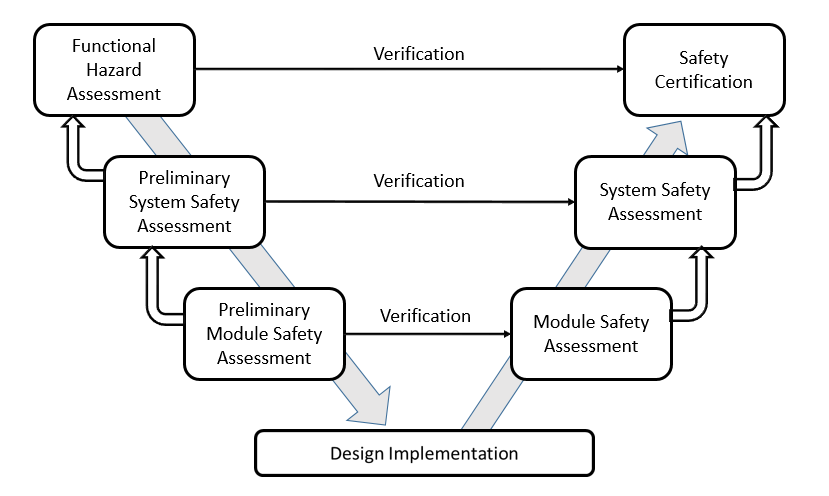
\includegraphics[width=0.85\textwidth] {images/v2.png}}
        \caption{\label{fig:v2} The V Model in Safety Assessment}
\end{figure}

The safety assessment shown in Figure~\ref{fig:v2} integrates each phase of the V model with analyses specific to system hazards and their severity. It also shows how these hazards should be addressed within the design phase. The safety assessment proess is defined in ARP4754A by the following phases:

\begin{description}
\item[Functional Hazard Assessment (FHA)] examines the functions of the system to identify potential functional failures and classifies the potential hazards associated with them. This includes identification of failure conditions, identifying the effects of those failures, classification of each failure condition, and assignment to safety objectives.

\item[Common Cause Analysis (CCA)] verifies and establishes physical and functional separation, isolation, and independence requirements between subsystems and verifies that these requirements have been met.

\item[Preliminary Aircraft Safety Assessment (PASA)] establishes aircraft safety requirements and provide a preliminary indication that the aircraft can meet those safety requirements.

\item[Preliminary System Safety Assessment (PSSA)] examines the proposed architecture(s) to determine how failures could cause the failure conditions determined by the FHA. The objective is to complete the safety requirements of an aircraft or system and show that the proposed system architecture satisfies the safety requirements. The PSSA is an iterative process that is performed at multiple stages of system development. 

\item[Fault Tree Analysis (FTA)] is performed to find combinations of faults that lead to the violation of a safety requirement. The fault tree itself shows the logical relation between the sets of faults and the violation of a safety requirement.

\item[Common Mode Analysis (CMA)] analyzes designs and implementations for elements that may defeat the redundancy
or independence of functions within the design, i.e. if elements are shown as independent in FTA, make sure they are truly independent in the system under consideration.

\item[Failure Modes and Effect Analysis (FMEA)] aims at finding the causality relationship between sets of faults, intermediate events, and undesired states in the system. Usually this is represented in tabular form and called an \textit{FMEA table}.

\item[Aircraft Safety Assessment (ASA)/System Safety Assessment (SSA)] verifies that the system (or aircraft), as implemented, meets the safety requirements specified by the PSSA.

\end{description}

\begin{comment}
\subsection{Proposed Model Based Safety Assessment Process Supported by Formal Methods}
We propose a model-based safety assessment process backed by formal methods to help safety engineers with early detection of the design issues.  This process uses a single unified model to support both system design and safety analysis; this is shown in Figure~\ref{fig:SACycle1} and is based on the following steps:

\begin{enumerate}
	\item System engineers capture the critical information in a shared model:  high-level hardware and software architecture, nominal behavior at the component level, and safety requirements at the system level.
	\item System engineers use a model checker to check that the safety requirements are satisfied by the nominal design model. 
	\item Safety engineers augment the nominal model with the component failure modes. In addition, safety engineers specify the fault hypothesis for the analysis which corresponds to how many simultaneous faults the system must be able to tolerate.
	\item Safety engineers use a model checker to analyze if the safety requirements and fault tolerance objectives are satisfied by the design in the presence of faults. If the design does not tolerate the specified number of faults (or probability threshold of fault occurrence), then the tool produces counterexamples or minimal sets of fault combinations that can cause the safety requirement to be violated.
	\item The safety engineers examine the results to assess the validity of the fault combinations and the fault tolerance level of the system design. If a design change is warranted, the model will be updated with the latest design change and the above process is repeated.
\end{enumerate}

\begin{figure}[h]
	\begin{center}
		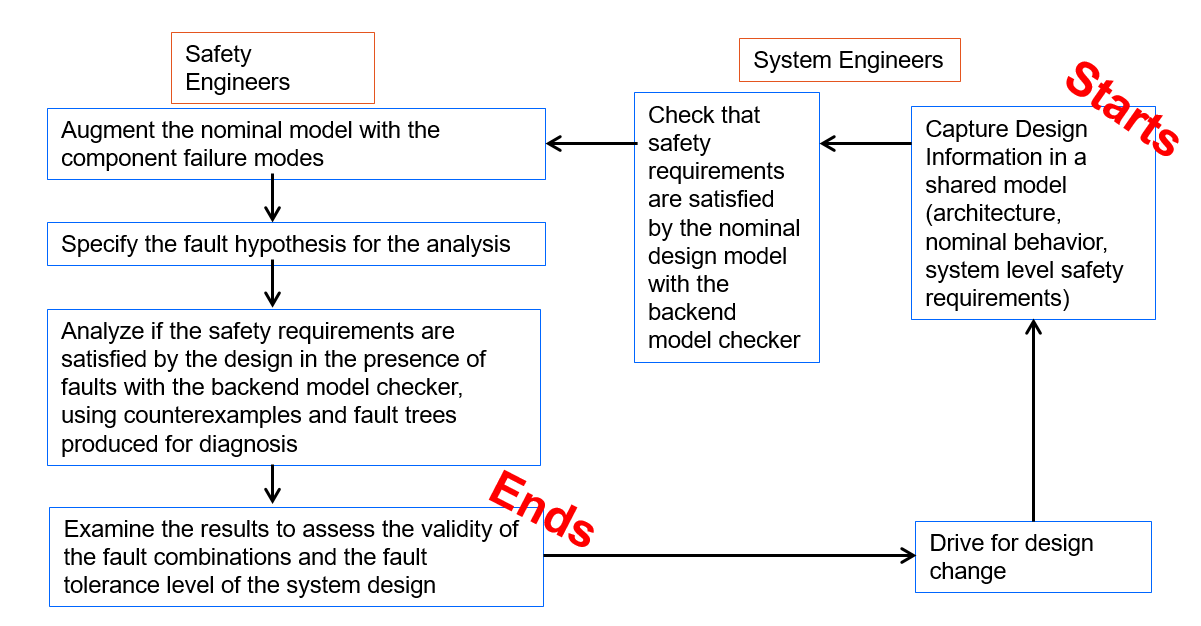
\includegraphics[width=\textwidth]{images/SACycle.PNG}
	\end{center}
	\caption{Proposed Steps of the Safety Assessment Process}
	\label{fig:SACycle1}
\end{figure}

These steps can be viewed as a cyclical process that involves both the system development engineers and the safety engineers of the system. Figure~\ref{fig:SACycle1} shows these steps within the context of the start and end of a project. 

\danielle{Add a bit more information here - pull from the MBSE project for IRAD. Include reasons why this approach is better, how it will help safety analysts, how it benefits the field as a whole. Then lead into the next sections with a statement about model checking, verification, etc.}
\end{comment}
\subsection{Fault Forests, Trees, and Minimal Cut Sets}
\label{sec:saArtifacts}
%\danielle{Move this paragraph to where it makes sense.} Safety analysis has traditionally been performed manually, but with the rise of model checking and the improvement of its capabilities, the world of safety analysis began to see its powerful benefits~\cite{hinchey2012industrial, liggesmeyer1998improving, coudert1993fault, Bozzano:2010:DSA:1951720,bozzano2003esacs}. There arose multiple ways of viewing the system and fault models, various ways of automating the capture of safety pertinent information, and a number of tools that addressed various issues that arose. In this section, we discuss the state of the practice and how formal methods has been applied in the domain of safety assessment research.

A \emph{fault tree} is a directed acyclic graph whose leaves model component failures and whose gates model failure propagation. The system failure under examination is the root of the tree and is called the \emph{top level event}. The \emph{basic events} are the events that can occur in the system which lead to the top level event and in the graphical model, these correspond to the leaves. A {\em fault forest} is simply a set of fault trees. The gates in the fault tree describe how failures propagate through the system. Each gate has one output and one or more inputs. In Figure~\ref{fig:introFT}, the AND gate has three inputs and one output. The leaves of the tree represent the basic events of the system and in the case of this fault tree, these three events are also a \textit{minimum cut set} for this top level event. The minimal cut set is the minimal set of basic events that must occur together in order to cause the top level event to occur. Finding these sets is important to fault tree analysis and has been an active area of interest in the research community since fault trees were first described in Bell Labs in 1961~\cite{historyFTA, 0f356f05e72f43018211b36f97c8854a}. 

\begin{figure}[h]
\begin{center}
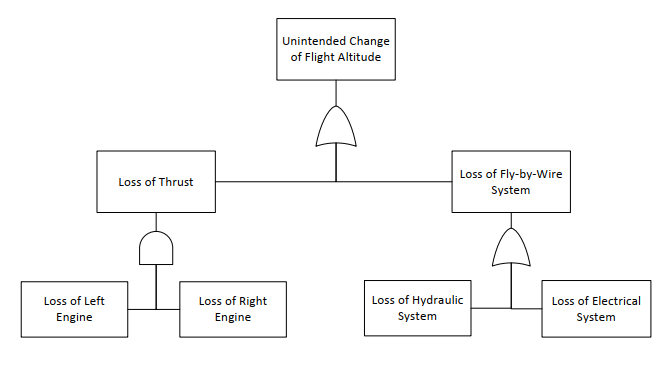
\includegraphics[width=8cm]{images/ft.png}
\caption{A Simple Fault Tree} \label{fig:introFT}
\end{center}
\end{figure}

Figure~\ref{fig:introFT} shows a simple example of a fault tree. In this example, the top level event corresponds to an aircraft having an unintended change of altitude. In order for this event to occur, there must be either a loss of thrust or the loss of a Fly-by-Wire system. This is seen through the use of the OR gate below the top level event. The malfunction of both the left and right engines will cause the loss of thrust to occur and the Fly-by-Wire system can be lost if either the hydraulic system or the electrical system were to malfunction. The MCSs for this example are \{Loss of Left Engine, Loss of Right Engine\}, \{Loss of Hydraulic System\}, and \{Loss of Electrical System\}. 

%There are two main types of FTA that we differentiate here as \textit{qualitative} analysis and \textit{quantitative} analysis. In qualitative analysis, the structure of the fault tree is considered and the cut sets are a way to indicate which combinations of component failures will cause the system to fail. On the other hand, in quantitative analysis the probability of the TLE is calculated given the probability of occurance of the basic events. 

\textbf{History of Fault Trees} 
Since the early days of safety engineering, fault tree analysis has been a primary method of determining safety of a system and showing the behavior of the system (with respect to its requirements) in the presence of faults~\cite{0f356f05e72f43018211b36f97c8854a,vesely1981fault}. Fault tree analysis requires one to explore the faults of the system and their effects on system behavior to determine minimal fault configurations that may violate requirements. From the beginning of fault tree analysis in the 1960s, algorithms worked directly with the fault tree structure to produce minimal cut sets~\cite{10020219108,semanderes1971elraft}. In essence, these algorithms represented each AND/OR gate as a boolean expression and then performed simplification to relate the basic events to the top level event without any gates~\cite{0f356f05e72f43018211b36f97c8854a}. In 1993, Rauzy et al. developed a new approach that converted the fault tree structure into a binary decision diagram (BDD)~\cite{rauzy1993new}. This was a natural way to reduce the Boolean formula into something far more computationally efficient and reducible to even simpler forms. BDDs are still commonly used to perform quantitative and qualitative fault tree analysis~\cite{sinnamon1997new,bryant1986graph,aralia1996computation,reay2002fault,rauzy2007assessment,ge2015quantitative,jiang2018algebraic,banov2019new}.  Other forms of fault tree analysis include Monte Carlo methods~\cite{vesely1970prep}, Markov chains~\cite{boudali2007dynamic}, and zero suppressed BDDs~\cite{minato2001zero}. 




\begin{comment}
\subsubsection{Failure Mode and Effects Analysis}
\danielle{Is this section necessary? If I don't talk about FMEA tables again, cut this.} Failure Mode and Effects Analysis (FMEA) was one of the first systematic ways of performing dependability analysis and is used throughout the safety critical industries~\cite{rausand2003system,Bozzano:2011:SDP:1992983.1992988}. FMEA provides a structured way to list possible failures and their consequences systemwide. If probabilities of failures are known, quantitative analysis can be performed to estimate system reliability and to assign critical significance to potential failure modes or system components~\cite{MilStandardFMEA}. Performing FMEA is often the first step in the fault tree construction, for it shows possible component failures and hence basic events~\cite{0f356f05e72f43018211b36f97c8854a}. Typically, the failure modes of the components at a given level are considered; the objective it to identify the effects of the failure modes at that level - and usually higher levels - of the design. The FMEA results are often presented in tabular form (FMEA Table). FMEA tables vary in form, but almost always include failure mode definitions, the operational mode in which the failure can occur, and possible causes of the failure~\cite{Bozzano:2010:DSA:1951720}.
\end{comment}

\subsection{Model Based Development}
\label{sec:mbd}
System safety analysis techniqes are well established and used extensively in the design of safety critical systems. These safety analysis techniques are often performed manually based on informal design models and various other documents~\cite{schatz2002model,Joshi05:Dasc}. Fault trees are one of the most common artifacts used by safety engineers, but different engineers may produce substantially different fault trees for the same system. It becomes clear that the analyses are highly subjective and dependent on the skill of the practitioner. Since the analyses are based on informal system documentation, researchers and practitioners have proposed a consolidation of the information into a central entity and use this to perform safety analysis~\cite{joshi2008behavioral, Joshi05:SafeComp, Joshi07:Hase, CAV2015:BoCiGrMa, Bozzano:2010:DSA:1951720, lisagor2011model}.

One way to achieve consolidation of information spread across various informal documents is through \emph{Model-based Development} (MBD)~\cite{schatz2002model}. In MBD, the development is centered around a formal specification or model of the system. This model can be analyzed for completeness and consistency~\cite{heimdahl1996completeness}, model checking~\cite{miller2010software,clarke2018model, grumberg1994model}, theorem proving~\cite{rayadurgam2003using}, test case generation~\cite{anand2013orchestrated,rayadurgam2001coverage}, etc. One can also automate aspects of the implementation from the formal specification. There are several modeling and verification notations that provide these capabilities. 

Model-based Development can also refer to a process that considers a non-formal model, such as SysML~\cite{friedenthal2014practical} or UML~\cite{fowler2003brief}, as the central development artifact. In this dissertation, we consider a formal model of the system in a language with well-defined semantics as the central artifact of the MBD process. 

While there are numerous modeling languages and specifications both in industry and research, we focus on one for this research: the Architecture Analysis and Design Language. 

\subsubsection{Architecture Analysis and Design Language}
The Architectural Analysis and Design Language (AADL) is an SAE International standard language that provides a unifying framework for describing the system architecture for performance-critical, embedded, real-time systems~\cite{AADL_Standard,FeilerModelBasedEngineering2012}. From its conception, AADL has been designed for the design and construction of avionics systems.  Rather than being merely descriptive, AADL models can be made specific enough to support system-level code generation.  
 
An AADL model describes a system in terms of a hierarchy of components and their interconnections, where each component can either represent a logical entity (e.g., application software functions, data) or a physical entity (e.g., buses, processors). An AADL model can be extended with language annexes to provide a richer set of modeling elements for various system design and analysis needs (e.g., performance-related characteristics, configuration settings, dynamic behaviors). The language definition is sufficiently rigorous to support formal analysis tools that allow for early phase error/fault detection. 

Further details regarding AADL will be introduced as needed throughout this dissertation. 
\subsection{Model Based Safety Assessment}
\label{subsec:mbsa}

The lack of precise models of the system architecture and its failure modes often forces safety analysts to devote significant effort to gathering architectural details about the system behavior from multiple sources. Furthermore, this investigation typically stops at system level, leaving software function details largely unexplored. Typically equipped with the domain knowledge about the system, but not detailed knowledge of how the software applications are designed, practicing safety engineers find it a time consuming and involved process to acquire the knowledge about the behavior of the software applications hosted in a system and its impact on the overall system behavior. A diagram of this process is shown in Figure~\ref{fig:proposed_safety_process}.

\begin{figure}[h]
	\centering
	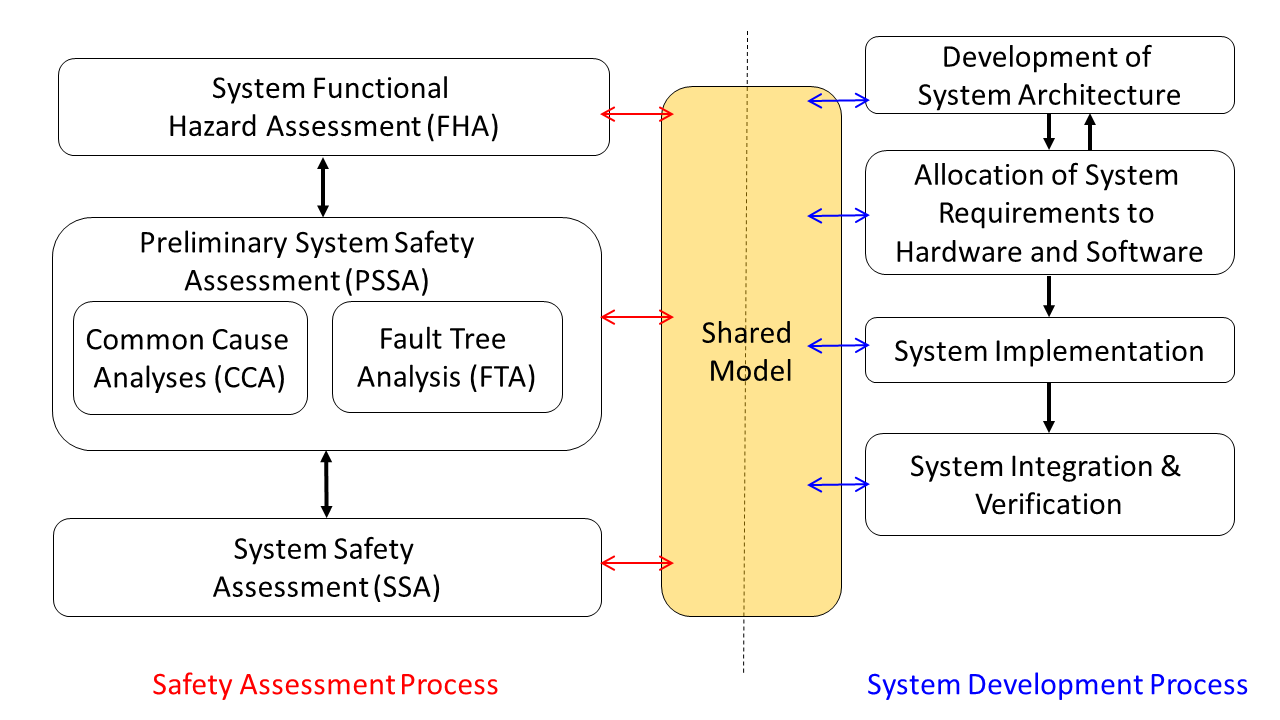
\includegraphics[trim=0 5 0 5,clip,width=0.85\textwidth]{images/process3.png}
	\caption{Use of the Shared System/Safety Model in the ARP4754A Safety Assessment Process}
	\label{fig:proposed_safety_process}
\end{figure}

Industry practitioners have come to realize the benefits of using models in the safety assessment process, and a revision of the ARP4761 to include Model Based Safety Analysis (MBSA) is under way. 

\subsection{Suggested Model Based Safety Assessment Process Supported by Formal Methods}
We propose a model-based safety assessment process backed by formal methods to help safety engineers with early detection of the design issues.  This process uses a single unified model to support both system design and safety analysis; this is shown in Figure~\ref{fig:SACycle1} and is based on the following steps:

\begin{enumerate}
	\item System engineers capture the critical information in a shared model:  high-level hardware and software architecture, nominal behavior at the component level, and safety requirements at the system level.
	\item System engineers use a model checker to check that the safety requirements are satisfied by the nominal design model. 
	\item Safety engineers augment the nominal model with the component failure modes. In addition, safety engineers specify the fault hypothesis for the analysis which corresponds to how many simultaneous faults the system must be able to tolerate.
	\item Safety engineers use a model checker to analyze if the safety requirements and fault tolerance objectives are satisfied by the design in the presence of faults. If the design does not tolerate the specified number of faults (or probability threshold of fault occurrence), then the tool produces counterexamples or minimal sets of fault combinations that can cause the safety requirement to be violated.
	\item The safety engineers examine the results to assess the validity of the fault combinations and the fault tolerance level of the system design. If a design change is warranted, the model will be updated with the latest design change and the above process is repeated.
\end{enumerate}

\begin{figure}[h]
	\begin{center}
		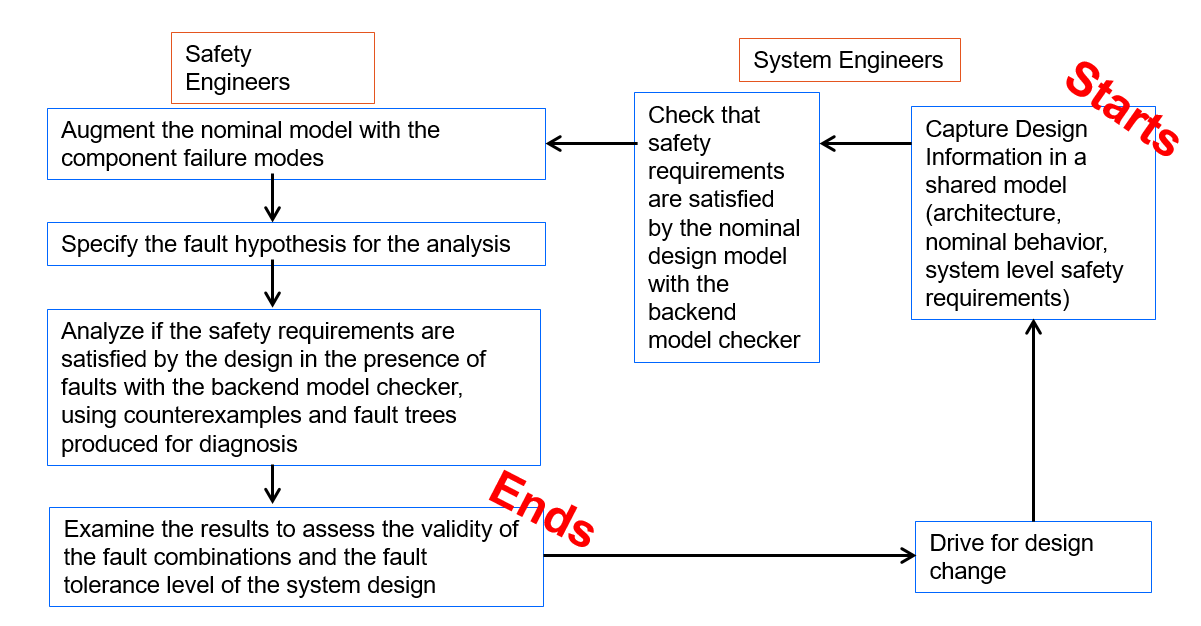
\includegraphics[width=\textwidth]{images/SACycle.PNG}
	\end{center}
	\caption{Proposed Steps of the Safety Assessment Process}
	\label{fig:SACycle1}
\end{figure}

These steps can be viewed as a cyclical process that involves both the system development engineers and the safety engineers of the system. Figure~\ref{fig:SACycle1} shows these steps within the context of the start and end of a project. 

\danielle{Add a bit more information here - pull from the MBSE project for IRAD. Include reasons why this approach is better, how it will help safety analysts, how it benefits the field as a whole. Then lead into the next sections with a statement about model checking, verification, etc.}

\section{Formal Methods}
\label{sec:fm}
As the complexity of systems increase, the cost of development and validation consumes more time and resources than ever before; nevertheless, these processes are vital in safety critical systems when the loss of functionality of the system can result in loss of life. Authorities have put in place various thresholds for the likelihood of such events and it is the responsibility of the system developers to show that undesirable events are sufficiently unlikely to occur~\cite{faaSA}. Utilizing the recent advancements in automated formal verification within the validation process has become essential to the certification of critical systems~\cite{deptOfDefense,standard1999,prasad2005survey} and the world of safety analysis began to see its powerful benefits~\cite{hinchey2012industrial, liggesmeyer1998improving, coudert1993fault, Bozzano:2010:DSA:1951720,bozzano2003esacs}. There arose multiple ways of viewing the system and fault models, various ways of automating the capture of safety pertinent information, and a number of tools that addressed practical issues. Formal validation and verification is a proof-based methodology used to assess the correctness of requirements, system design, and implementation. This section provides a background of the formal method techniques that are commonly used in the system development and safety assessment processes.

\subsection{Overview}
Given that this research is focused on model-based system development and safety assessment, we focus our attention onto \emph{model checking} as a method of formal analysis. Model checking is an automatic technique for verifying that system models meet their specified requirements~\cite{clarke2018model}.  Applying model checking to a system design consists of a few main tasks: \emph{modeling}, \emph{formal specification}, and \emph{formal verification}. The digital and mechanical components of a system can be described in abstract form (modeling), and the requirements of the system and of each component can be specified in formal logic (formal specification). Formal verification is demonstrating that the model satisfies its specification using math. The verification of a model takes both the design and the requirement specification into account when analyzing the behavior and interactions of the components. In the sections that follow, we will outline these three major components of model checking and describe the aspects important in this research.

\subsection{Modeling}
\label{sec:modeling}
When modeling a system, the digital and mechanical components are described in abstract form; furthermore, the requirements of the system and of each component can be specified in formal logic. The verification of such models take both the architecture and the requirement specification into account when analyzing the behavior and interactions of the components comprising the system. Throughout the past few decades, numerous modeling languages and tools have been introduced, for example Simulink from MathWorks~\cite{MathWorks}, SCADE from Esterel Technologies~\cite{abdulla2004designing}, and research base languages such as Lustre~\cite{Halbwachs91:IEEE}. Other common modeling languages include SysML~\cite{friedenthal2014practical} and AADL~\cite{FeilerModelBasedEngineering2012}. 

Often, engineers who design safety critical systems model their systems as networks of operators transforming flows of data. At a higher level, this can be represented by block diagrams that group these networks into reusable components. {\em Dataflow} languages allow these models to directly represent the digital control system. Dataflow programming languages have several merits, one of which is that the program is a completely functional model of the system. This feature makes the model well suited to formal verification and program transformation; it also facilitates reuse, because the module will behave the same way in any context into which it is embedded~\cite{joshi2008behavioral}. For this dissertation, we focus our attention on Lustre~\cite{Halbwachs91:IEEE}, a synchronous\footnote{A synchronous language breaks real time into a sequence of instants in which the outputs of the model are computed.} dataflow programming language used in the formal verification portion of this research. Lustre is described in more detail in Section~\ref{sec:lustre}. 




\begin{comment}
\subsubsection{Ordered Binary Decision Diagrams}
A Binary Decision Diagram (BDD) is a data structure used to encode Boolean formulae.
\begin{figure}[htbp]
        \center{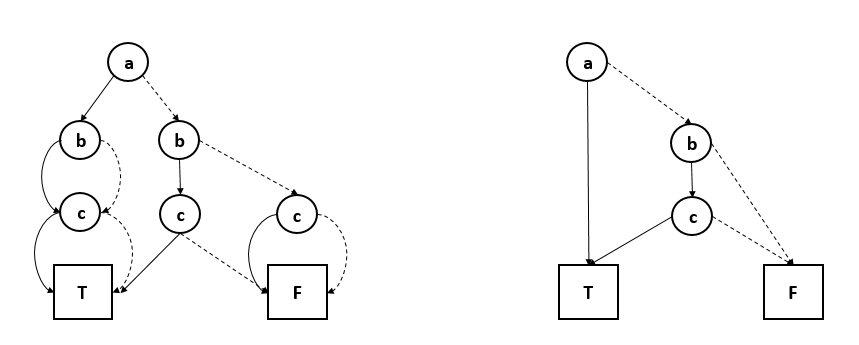
\includegraphics[width=0.8\textwidth] {images/bdd.png}}
        \caption{\label{fig:bdd} Binary Decision Diagrams of the Formula $a \lor (b \land c)$}
\end{figure}
As shown in Figure~\ref{fig:bdd}, it is a rooted, directed, acyclic graph with internal decision nodes and two terminal nodes (\textit{true} and \textit{false}). Each of the decision nodes is labeled with a Boolean variable and has two child nodes, low child and high child. The edge from a node to its low child represents the assignment of \textit{false}, likewise the edge to the high child represents the assignment of \textit{true}. The BDD is called \textit{ordered} if different variables appear in the same order on all paths from the root. Intuitively, following a path from the root to the \textit{true} terminal node represents a valid assignment to the Boolean formula (invalid in the case of ending on the \textit{false} terminal node). 

BDDs are reduced by the removal of isomorphic subgraphs. The BDD shown on the right of Figure~\ref{fig:bdd} is the reduced form of the BDD on the left.
\end{comment}


\subsection{Formal Specification}
\label{sec:formalSpec}
Before we can verify the correctness of a system, we must first specify the properties that the system should have~\cite{clarke2018model}. The formal specification process translates the informal system requirements into a mathematical logic to determine if the system design is correct~\cite{hinchey2012industrial}. This process guarantees an unambiguous description of the requirements, which is not possible when using an informal natural language. The formal definition of system requirements includes the system design and its expected behavior as well as the assumptions on the environment in which the system is expected to operate. A design or implementation can never be considered correct in isolation; it is only correct with respect to the specifications. The expected behavior, system design, and environmental assumptions change and are refined as the system goes through the various stages of development~\cite{lamsweerde2000formal}. A commonly used method of specification is \emph{temporal logic}. Temporal logics are useful for specifying complex system requirementss, because they can describe the ordering of events in time without introducing time explicitly. 

\subsubsection{Linear Temporal Logic}
Temporal logic can be used to express properties of reactive systems~\cite{Bozzano:2010:DSA:1951720}. System properties are usually classified into two main categories: {\em safety properties} and {\em liveness properties}. Safety properties express the idea that ``nothing bad ever happens" where liveness properties state that ``something good will eventually happen." 

An example of a safety property is: ``it is never the case that the brake pedal is pressed and no hydraulic pressure is supplied at the wheel." A liveness property, on the other hand, could state: ``eventually the process will complete its execution." 

Traditionally, two types of temporal logic are used in model checking; Computational Tree Logic (CTL), which is based on a branching time logic model, and Linear Temporal Logic (LTL), based on a linear representation of time. This research will focus on LTL. 

An LTL formula is built from a set of atomic propositions, logical operators, and basic temporal operators. The formula is evaluated over a linear path or sequence of states, $s_0, s_1, ..., s_i ,s_{i+1},...$. The following temporal operators are provided:
\begin{itemize}
    \item Globally (\textbf{G}): $G_p$ is true in a state $s_i$ if and only if $p$ is true in all states $s_j$ with $j \geq i$.
    
    \item Finally (\textbf{F}): $F_p$ is true in state $s_i$ if and only if $p$ is true in some state $s_j$ with $j \geq i$.
    
    \item Next (\textbf{X}): $X_p$ is true in state $s_i$ if and only if $p$ is true in the state $s_{i+1}$. 
    
    \item Until (\textbf{U}): $pUq$ is true in state $s_i$ if and only if $q$ is true in some state $s_j$ with $j \geq i$ and $p$ is true in all states $s_k$ such that $i \leq k < j$.
\end{itemize}

Other temporal operators can be defined on the basis of the operators above~\cite{sistla1985complexity}. Formal definitions and more information on LTL and CTL can be found in a number of research works~\cite{Bozzano:2010:DSA:1951720, clarke2018model}.

\subsection{Formal Verification} 
\label{sec:formalVer}
Once we have specified the important properties (formal specification), then a formal model for the system is created; this model captures the properties that must be considered to establish correctness~\cite{clarke2018model}; this process is referred in this dissertation as \emph{formal verification}. Formal verification is the use of proof methods to show that given the environmental assumptions stated in the formal specification, the formal design of the system meets the requirements. The problem can be reduced to that of property checking: given a program $P$ and a specific property, does the program satisfy the given property~\cite{fitting2012first}.  

Model checking was introduced in the early 1980s and consists of exploring the states and transitions of a model~\cite{clarke1981design,queille1982specification}. By representing the system abstractly, a possibly infinite state space is reduced to a finite model.~\cite{d2008survey}. The proofs are generated over an abstract mathematical model of the system, such as finite state machines, labeled transition systems, or timed automata. It takes as input a model of a system and the properties written in formal logic, then explores the state space of the system to determine if the model violates the properties~\cite{clarke2018model,fraser2009testing}. In recent years, model checking takes advantage of abstraction techniques specific to a domain to consider multiple states or transitions in a single operation; this lessens computation time considerably~\cite{d2008survey}. Nevertheless, the biggest limiting factor of model checking is scalability and much of the recent research in this area attempts to address this problem~\cite{clarke2018model}.

Deductive methods of verification consists of generating proof obligations from the specifications of the system and using these obligations in a theorem prover setting. Automated theorem provers have the main objective to show that some statement (conjecture) is a logical consequence of other statements (the axioms and hypotheses). The rules of inference are given as are the set of axioms and hypotheses~\cite{d2008survey,fitting2012first}. Deductive methods of verification include automated theorem provers (e.g., Coq~\cite{coq}, Isabelle~\cite{isabelle}) and satisfiability modulo theories (e.g., SMTInterpol~\cite{smtInterpol}, Z3~\cite{z3}, Yices~\cite{yices}). 



%\subsection{Modeling}
\label{sec:modeling}
When modeling a system, the digital and mechanical components are described in abstract form; furthermore, the requirements of the system and of each component can be specified in formal logic. The verification of such models take both the architecture and the requirement specification into account when analyzing the behavior and interactions of the components comprising the system. Throughout the past few decades, numerous modeling languages and tools have been introduced, for example Simulink from MathWorks~\cite{MathWorks}, SCADE from Esterel Technologies~\cite{abdulla2004designing}, and research base languages such as Lustre~\cite{Halbwachs91:IEEE}. Other common modeling languages include SysML~\cite{friedenthal2014practical} and AADL~\cite{FeilerModelBasedEngineering2012}. 

Often, engineers who design safety critical systems model their systems as networks of operators transforming flows of data. At a higher level, this can be represented by block diagrams that group these networks into reusable components. {\em Dataflow} languages allow these models to directly represent the digital control system. Dataflow programming languages have several merits, one of which is that the program is a completely functional model of the system. This feature makes the model well suited to formal verification and program transformation; it also facilitates reuse, because the module will behave the same way in any context into which it is embedded~\cite{joshi2008behavioral}. For this dissertation, we focus our attention on Lustre~\cite{Halbwachs91:IEEE}, a synchronous\footnote{A synchronous language breaks real time into a sequence of instants in which the outputs of the model are computed.} dataflow programming language used in the formal verification portion of this research. Lustre is described in more detail in Section~\ref{sec:lustre}. 




\begin{comment}
\subsubsection{Ordered Binary Decision Diagrams}
A Binary Decision Diagram (BDD) is a data structure used to encode Boolean formulae.
\begin{figure}[htbp]
        \center{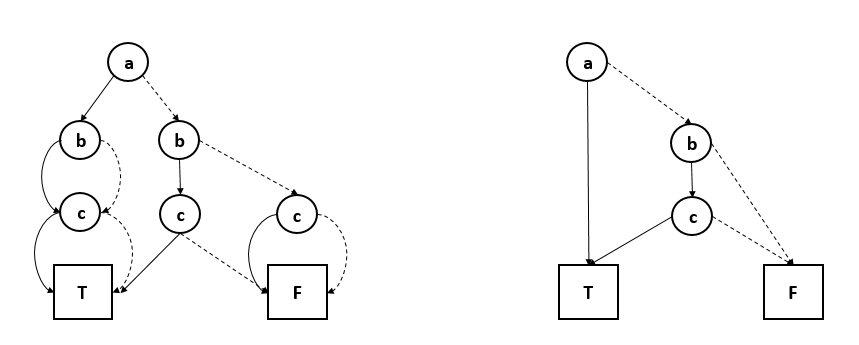
\includegraphics[width=0.8\textwidth] {images/bdd.png}}
        \caption{\label{fig:bdd} Binary Decision Diagrams of the Formula $a \lor (b \land c)$}
\end{figure}
As shown in Figure~\ref{fig:bdd}, it is a rooted, directed, acyclic graph with internal decision nodes and two terminal nodes (\textit{true} and \textit{false}). Each of the decision nodes is labeled with a Boolean variable and has two child nodes, low child and high child. The edge from a node to its low child represents the assignment of \textit{false}, likewise the edge to the high child represents the assignment of \textit{true}. The BDD is called \textit{ordered} if different variables appear in the same order on all paths from the root. Intuitively, following a path from the root to the \textit{true} terminal node represents a valid assignment to the Boolean formula (invalid in the case of ending on the \textit{false} terminal node). 

BDDs are reduced by the removal of isomorphic subgraphs. The BDD shown on the right of Figure~\ref{fig:bdd} is the reduced form of the BDD on the left.
\end{comment} % TS
%\input{modelchecking} %ltl, etc
%\subsubsection{The SAT Problem and SMT Solvers}
\label{sec:satsmt}
The Boolean Satisfiability (SAT) problem attempts to determine if there exists a total truth assignment to a given propositional formula, that evaluates to $true$. Generally, a propositional formula is any combination of the disjunction and conjunction of literals (as an example, $a$ and $\neg a$ are literals). For example, the proposition $a \land b$ is satisfiable; when $a$ and $b$ are assigned to $true$, the formula is satisfied, or true.  On the other hand, the proposition $a \land \neg a$ is unsatisfiable; no such assignment can be found to satisfy both $a$ and $\neg a$. 

Satisfiability Modulo Theories (SMT) solvers also address the SAT problem, but can work over propositional logic or predicate logic with quantifiers. An SMT solver works over a conjunction of literals, as is the case with SAT solvers, but the literals can be expressed as predicates over non-boolean variables, such as $x > 0$. A boolean literal can be satisfied with a finite number of possible assignments; this is not always the case with an SMT formula.


\textbf{UNSAT Cores and Minimal Unsatisfiable Subsets}
When analyzing a model, there are certain questions that may be asked about the model requirements. If a model is unsatisfiable with respect to some system level property, it is of benefit to know \emph{why} it is not satisfiable. 

A constraint system $C$ is an ordered set of $n$ abstract constraints $\{C_1, C_2, ..., C_n\}$ over a set of variables. The constraint $C_i$ restricts the allowed assignments of these variables in some way~\cite{liffiton2016fast}. Given a constraint system, we require some method of determining, for any subset $S \subseteq C$, whether $S$ is \textit{satisfiable} (SAT) or \textit{unsatisfiable} (UNSAT). Given a constraint system $C$, there are certain subsets of $C$ that are of interest in terms of satisfiability. Definitions 2-4 are taken from research by Liffiton et. al.~\cite{liffiton2016fast}. 

For a given unsatisfiable problem, SAT solvers (and SMT solvers) attempt to provide proof of unsatisfiability by providing a subset of UNSAT clauses known as \textit{UNSAT cores}. In general, this is useful information to have regarding the constraint system in question. 

\begin{definition} A Minimal Unsatisfiable Subset (MUS) $M$ of a finite constraint system $C$ is a subset $M \subseteq C$ such that $M$ is unsatisfiable and $\forall c \in M$ : $M \setminus \{c\}$ is satisfiable. 
\end{definition}

\begin{definition} UNSAT core: Let $C$ be a finite set of constraints and $U \subseteq C$ an unsatisfiable subset. A constraint $c \in U$ is an UNSAT core for $U$ if $U \setminus \{c\}$ is satisfiable. A set of all unsatisfiability cores of $U$ constitute an MUS for $C$. 
\end{definition}

Intuitively, an MUS is the minimal explanation of the constraint systems infeasability and the UNSAT cores are the building blocks of the MUS. In recent years, a number of efficient algorithms have been introduced to find MUSs~\cite{liffiton2005max} and most of them focus on finding a single such subset~\cite{belov2012towards, belov2013core, belov2012muser2}. More recently, algorithms have been introduced that can find all such minimal unsatisfiable subsets~\cite{GhassabaniGW16, Ghassabani2017EfficientGO,bendik2018online}. 


\textbf{Inductive Validity Cores} Given a complex model, it is useful to extract traceability information related to the proof; in other words, which elements of the model were necessary to construct the proof of a safety property. An algorithm was introduced by Ghassabani et al. to provide Inductive Validity Cores (IVC) as a way to determine which model elements are necessary for the inductive proofs of the safety properties for sequential systems~\cite{GhassabaniGW16}. Given a safety property of the system, a model checker is invoked to construct a proof of the property. The IVC generation algorithm extracts traceability information from the proof process and returns a minimal set of the model elements required in order to prove the property. Later research extended this algorithm in order to produce all minimal IVC elements (\aivcalg)~\cite{Ghassabani2017EfficientGO,bendik2018online}. 

The \aivcalg algorithm considers a constraint system consisting of the assumptions and contracts of system components and the negation of the safety property of interest (i.e. the top level event). It then collects all Minimal Unsatisfiable Subsets (MUSs) of this constraint system; these are the minimal explanations of the constraint systems infeasibility in terms of the \textit{negation} of the safety property. Equivalently, these are the minimal model elements necessary to prove the safety property. 

 

%\subsection{Compositional Model Checking and AGREE}
\label{compModelChecking}
Compositional analysis of systems was introduced in order to address the scalability of model checking large software systems~\cite{pnueli1985transition, heckel1998compositional, NFM2012:CoGaMiWhLaLu}. Normally, a SAT solver will flatten the hierarchical system model and use all model elements from all layers in order to find proof of a safety property. The analysis can alternatively be performed compositionally following the architecture hierarchy such that analysis at a higher level is based on the components at the next lower level and conducted layer by layer; the components of a system are organized hierarchically and each layer of the architecture is viewed a system. The idea is to partition the formal analysis of a system architecture into verification tasks that correspond into the decomposition of the architecture. 

\subsubsection{Assume-Guarantee Reasoning Environment}
The Assume-Guarantee Reasoning Environment (AGREE)~\cite{cofer2012compositional} provides a way to perform compositional verification on models that are defined using the Architecture Analysis and Design Language (AADL)~\cite{aerospace2012sae}. 

A component contract in an assume-guarantee reasoning environment is an assume-guarantee pair. Intuitively, the meaning of a pair is: if the assumption is true, then the component will ensure that the guarantee is true. The formulation of AGREE uses LTL operators $G$ (globally), $H$ (historically), and $Z$ (in the previous instant).

Formally, a component contract is an assume-guarantee pair $(A,P)$ for propositions $A, P$. The meaning of a pair is that a component is required to meet it's guarantee only if its assumptions have been true up to the current instant~\cite{cofer2012compositional}. Stated as an LTL formula, this is $G(H(A) \implies P)$. 

Each architectural layer is viewed as a system with inputs, outputs, and components. A system $S$ can be described as its own contract $(A_S, P_S)$ and the contracts of its components $C_S$. Thus, $S = (A_S, P_S, C_S)$. For each layer, the proof consists of demonstrating that the system guarantee is provable given the guarantees of its direct subcomponents and the system assumptions, or more formally prove $G(H(A_S) \implies P_S)$ given $G(H(A_C) \implies P_C)$ for each component $C$ in the system.  

This proof is performed one layer at a time starting from the top level of the system. When compared to monolithic analysis (i.e., analysis of the flattened model composed of all components), the compositional approach allows the analysis to scale to much larger systems~\cite{NFM2012:CoGaMiWhLaLu}. AGREE utilizes the JKind model checker~\cite{2017arXiv171201222G}, an infinite state $k$-induction model checker. Verification of the program is performed using a back-end SMT solver, e.g., Z3~\cite{z3}, SMTInterpol~\cite{smtInterpol}. 

\section{Formal Methods in Safety Analysis: A Brief History and the State of the Practice}
\label{sec:modelCheckingInSA}
Safety analysis has traditionally been performed manually, but with the rise of model checking and the improvement of its capabilities, the world of safety analysis began to see its powerful benefits~\cite{hinchey2012industrial, liggesmeyer1998improving, coudert1993fault, Bozzano:2010:DSA:1951720,bozzano2003esacs}. There arose multiple ways of viewing the system and fault models, various ways of automating the capture of safety pertinent information, and a number of tools that addressed various issues that arose. In this section, we discuss the state of the practice of related work and how formal methods has been applied in the domain of safety assessment research.

\subsection{Model Checking in Model Based Safety Analysis}
From the beginnings of model checking, there was a slow increase in its application to the domain of safety analysis, but a few research groups contributed immensely to this branch of study. Separately, these researchers began to contribute to safety analysis through the use of formal methods in the '90s and are still contributing today (e.g., \cite{reese1997software,signoret1998altarica,chiappini1999formal,cimatti2000industrial}. 

One of the main methods was the abstraction of the system into a formal transition system; this provided a means of defining a precise mathematical model of the system and simplifying mathematical operations through the use of abstraction techniques on the transition system. This helped to shrink the entire state space into something more digestible by computational techniques~\cite{d2008survey}. 

In the early 2000s, model based safety assessment began to make an appearance in literature~\cite{Bozzano:2010:DSA:1951720,Joshi05:Dasc, Joshi05:SafeComp, Joshi07:Hase}. The researchers began applied model checking in model based system development to safety analysis.  In this approach, a safety analysis system model is the central artifact in the safety analysis process, and traditional safety analysis artifacts, such as fault trees, are automatically generated by tools that analyze the system model.

The contents and structure of the safety analysis system model differ significantly across different conceptions of model-based safety analysis.  We can draw distinctions between approaches along several different axes.  The first is whether they propagate errors explicitly through user-defined propagations, which we call {\em explicit propagation}, or through behavioral requirements and interactions in the model itself, which we call {\em implicit propagation}.  The next is whether models and notations are {\em purpose-built} for safety analysis vs. those that extend {\em existing system models}.

For implicit propagation approaches, there are several additional dimensions.  One dimension involves whether {\em causal} or {\em non-causal} models are allowed.  Non-causal models allow simultaneous (in time) bi-directional error propagations, which allow more natural expression of some failure types (e.g. reverse flow within segments of a pipe), but are more difficult to analyze.  A final dimension involves whether analysis is {\em compositional} across layers of hierarchically-composed systems or {\em monolithic}.  

\begin{figure}[h]
	\begin{center}
		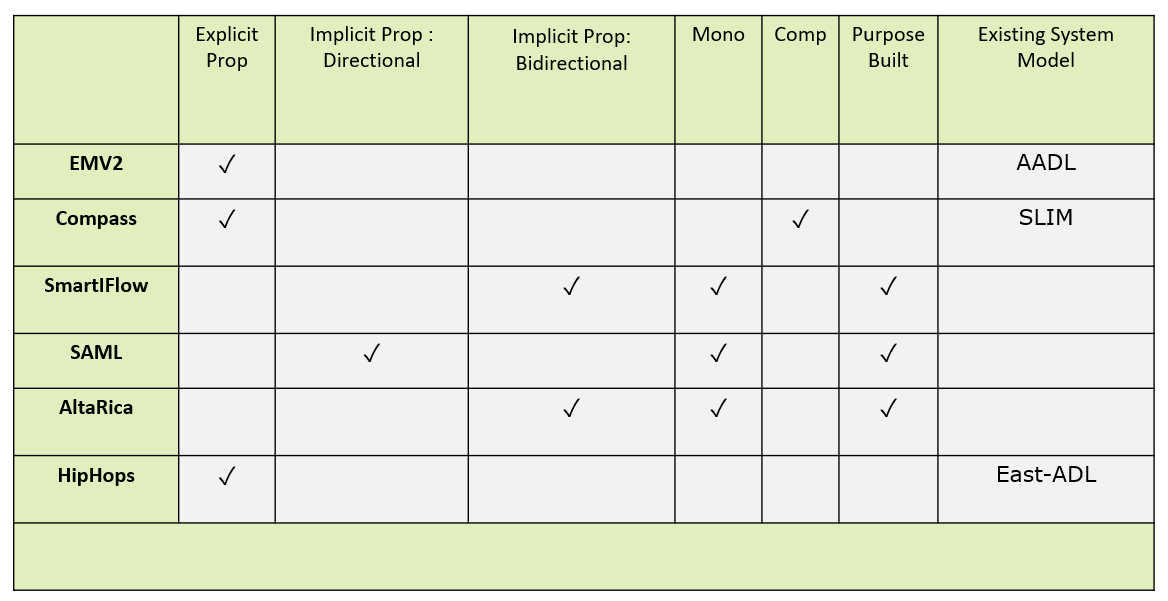
\includegraphics[width=\textwidth]{images/relatedWork.PNG}
	\end{center}
	\caption{Approaches of Related Work}
	\label{fig:relatedWork}
\end{figure}

Figure~\ref{fig:relatedWork} highlights the differences between these approaches in closely related work. The left column of the figure shows the tool names and across the top row are the various ways of structuring and analyzing the safety analysis system model. The tools and their approaches are described in the following subsections. 

These tools attempt to address various needs in the safety community and do so in distinct ways, but we wish to combine many of these efforts under one existing system model. We make it possible to extend the AADL system model with a fault model. Both nominal and fault analysis should be able to be performed monolithically or compositionally, and the fault model should allow for either explicit or implicit propagation. We attempt to address multiple needs within a single framework, unlike many of the related tools. 

This literature overview is not a complete account of all safety analysis model checking tools available either in industry or research, but highlights some of the most influential safety assessment methods and tools currently available. 

\subsubsection{AltaRica}
AltaRica was one of the first model checking tools specifically aimed at safety analysis of critical systems. The first iteration of AltaRica (1.0) performed over a transition system of the model, used dataflow ({\em causal}) semantics, and could capture the hierarchy of a system~\cite{signoret1998altarica}. The key idea was that this transition system (more specifically {\em constraint automata}) could be compiled into Boolean formulae and transformed into a binary decision diagram~\cite{point1999altarica}. The literature for performing fault tree analysis over BDDs was rich with algorithms; this was how much of the safety analysis artifacts were generated. The dataflow dialect (AltaRica 1.0) has substantial tool support, including the commercial Cecilia OCAS tool from Dassault~\cite{bieber2004safety}. For this dialect, the safety assessment, fault tree generation, and functional verification can be performed with the aid of NuSMV model checking~\cite{symbAltaRica}.

The most recent language update (AltaRica 3.0) uses non-causal semantics~\cite{prosvirnova2013compilationfaulttrees,prosvirnova2015automated,PROSVIRNOVA2013127}. Failure states are defined throughout the system and flow variables are updated through the use of assertions~\cite{Bieber04safetyassessment}.  AltaRica 3.0 has support for simulation and Markov model generation through the OpenAltaRica (www.openaltarica.fr) tool suite; it uses {\em implicit error propagation}, and it is a {\em purpose-built}, {\em monolithic} safety analysis language. 

\subsubsection{FSAP, xSAP, and COMPASS}
The Formal Safety Analysis Platform (FSAP) was introduced in 2003~\cite{bozzano2003improving} and supported failure mode definitions, safety requirements in temporal logic formulae, automated fault tree construction, and counterexample traces. The platform used NuSMV, a binary decision diagram (BDD)-based model checker~\cite{Cimatti2000}. The system model, written in NuSMV, and the fault model, developed graphically in FSAP, are together translated into a finite state machine and eventually into a BDD; fault tree analysis is performed using BDD algorithms implemented in NuSMV. 

By 2016, the researchers that developed FSAP (Foundation Bruno Kessler, FBK) released a similar tool called xSAP~\cite{DBLP:conf/tacas/BittnerBCCGGMMZ16}. xSAP extends FSAP in many ways: xSAP can handle infinite state machines, it is textual language rather than graphical, allows for richer fault modeling and definitions, and implements more than just BDD computations (e.g., SAT- and SMT-based routines). xSAP was integrated into the COMPASS toolsuite to take advantage of the algorithms it supports. More complex SAT-based algorithms were introduced to bypass the BDD method of minimal cut set generation, namely the ``anytime approximation" algorithms~\cite{CAV2015:BoCiGrMa, mattarei2016scalable}. These algorithms make clever use of bounded model checking algorithms to explore counterexamples provided to the query "the top level event never occurs." These explorations are done such that the cut sets generated are of increasing cardinality which allows for an approximation computation to be given even when the state space is too large to compute all minimal cut sets. These are implemented in xSAP~\cite{CAV2015:BoCiGrMa}.

COMPASS (Correctness, Modeling project and Performance of Aerospace Systems)~\cite{10.1007/978-3-642-04468-7_15} allows for {\em explicit propagation}, and is a {\em causal} {\em compositional} tool suite that uses the SLIM language, which is based on a subset of the Architecture Analysis and Design Language (AADL), for its input models~\cite{5185388, criticalembeddedsystems}. In SLIM, a nominal system model and the error model are developed separately and then transformed into an extended system model.  This extended model is automatically translated into input models for the NuSMV model checker~\cite{Cimatti2000, NuSMV}, MRMC (Markov Reward Model Checker)~\cite{Katoen:2005:MRM:1114692.1115230, MRMC}, and RAT (Requirements Analysis Tool)~\cite{RAT}. The safety analysis tool xSAP~\cite{DBLP:conf/tacas/BittnerBCCGGMMZ16} can be invoked in order to generate safety analysis artifacts such as fault trees and FMEA tables~\cite{compass30toolset}.  %COMPASS is an impressive tool suite, but some of the features that make AADL suitable for SW/HW architecture specification: event and event-data ports, threads, and processes, appear to be missing, which means that the SLIM language may not be suitable as a general system design notation (ESM).

\subsubsection{SmartIFlow}
SmartIFlow~\cite{info17:HaLuHo,honig2014new} uses {\em implicit propagation} and is a {\em purpose-built}, {\em monolithic} {\em non-causal} safety analysis tool that describes components and their interactions using finite state machines and events. Verification is done through an explicit state model checker which returns sets of counterexamples for safety requirements in the presence of failures.  SmartIFlow allows {\em non-causal} models containing simultaneous (in time) bi-directional error propagations.  On the other hand, the tools do not yet appear to scale to industrial-sized problems, as mentioned by the authors: ``As current experience is based on models with limited size, there is still a long way to go to make this approach ready for application in an industrial context''~\cite{info17:HaLuHo}.

\subsubsection{SAML}
The Safety Analysis and Modeling Language (SAML)~\cite{Gudemann:2010:FQQ:1909626.1909813} uses {\em implicit propagation}, and is a {\em purpose-built}, {\em monolithic} {\em causal} safety analysis language that was developed in 2010.  System models constructed in SAML can be used used for both qualitative and quantitative analyses. It allows for the combination of discrete probability distributions and non-determinism. The SAML model can be automatically imported into several analysis tools like NuSMV~\cite{Cimatti2000}, PRISM (Probabilistic Symbolic Model Checker)~\cite{CAV2011:KwNoPa}, or the MRMC model checker~\cite{Katoen:2005:MRM:1114692.1115230}. SAML itself does not provide the formal verification engines, but instead provides a platform to model the safety aspects of a system and then translate this into the input language for a formal verification engine~\cite{Gudemann:2010:FQQ:1909626.1909813}.

\subsubsection{Error Model Annex for AADL}
The SAE (Society of Automotive Engineers) released the
aerospace standard AS5506, named Architecture Analysis and Design Language (AADL), which is a mature industry-standard for embedded systems and has proved to be efficient for architecture modeling~\cite{aerospace2012sae,liu2016research}. AADL supports safety analysis by adding EMA (Error Model Annex) as an extension to the language. EMA allows the user to annotate system hardware and software architectures with hazard, error propagation, failure modes and effects due to failures. Around 2016, Version 2 of the Error Model Annex was released (EMV2)~\cite{EMV2}. EMV2 uses {\em explicit propagation} and is based on an {\em existing system model} approach. The faults and error propagations are explicitly defined and the fault tree analysis is performed by traversing propagation paths in reverse to find the original fault that caused the problem~\cite{feiler2017automated}. 


 % related work


%%%  Old section organization
%\section{Safety Critical Systems Development}
\label{sec:criticalSysDev}
As the capabilities of technology grows, so does the complexity and capabilities of mechanical and electrical systems. Many of these systems are safety critical; the loss of correct functioning leads to loss of life, substantial material or environmental damage, or large monetary losses. The development of such complex systems requires a process with clearly defined design and implementation phases which are subdivided into several sub-processes and phases. Certain sets of analyses are required for each of the phases and when the analyses provide satisfactory outcomes, the process transitions into the next phase. 

In general, each field relies on various interpretations of the development process. In the field of aerospace technologies, the Aerospace Recommended Practice (ARP) is what is commonly used. The Society of Automotive Engineers (SAE) is an association of engineers and professionals devoted to the standards that guide the development of transportation systems~\cite{SAE:ARP4761, SAE:ARP4754A}. 

\subsection{The V Model}
The development of safety critical systems is theoretically guided by the V model process as defined in ARP4754~\cite{SAE:ARP4754A}. The V model relates steps of the design phase with a post-implementation phase. It describes how the requirements are produced in the design phase and then how those requirements are verified against the implementation in the post-implementation phase. The left side of the V describes the requirements, architecture, and expected component behavior of the system (see Figure~\ref{fig:v1}). The right side of the V describes the evaluation of the system implementation in light of the requirements. 

\begin{figure}[!htb]
        \center{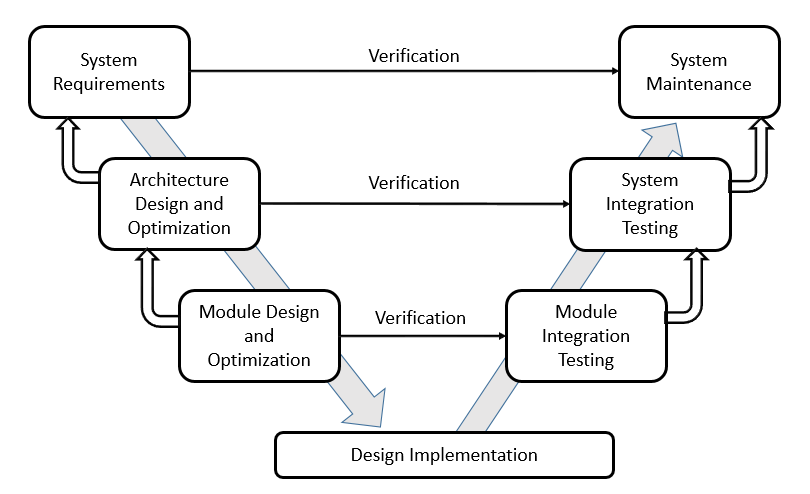
\includegraphics[width=0.85\textwidth] {images/v1.png}}
        \caption{\label{fig:v1} The V Model in System Development}
\end{figure}

\subsection{Traditional Safety Assessment Process}
ARP4754A, the Guidelines for Development of Civil Aircraft and Systems~\cite{SAE:ARP4754A}, provides guidance on applying development assurance at each hierarchical level throughout the development life cycle of highly-integrated/complex aircraft systems. It has been recognized by the Federal Aviation Administration (FAA) as an acceptable method to establish the assurance process. The safety assessment process is a starting point at each hierarchical level of the development life cycle and is tightly coupled with the system development and verification processes. It is used to show compliance with certification requirements and for meeting a company's internal safety standards. 

\begin{figure}[!htb]
        \center{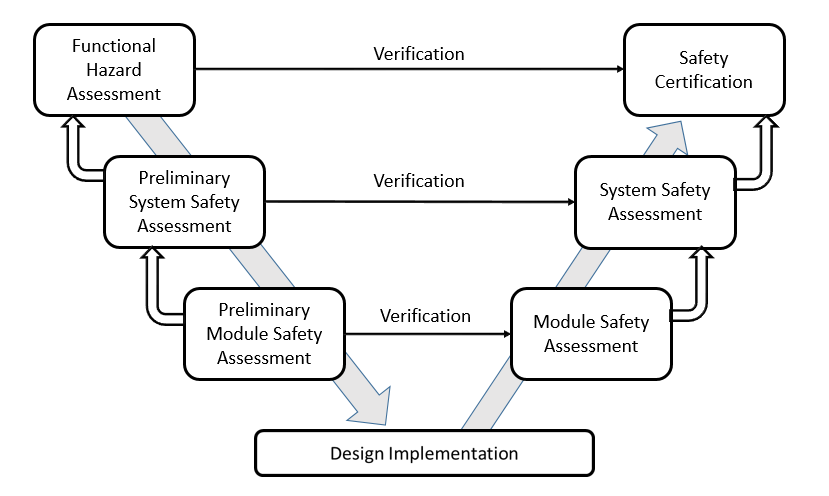
\includegraphics[width=0.85\textwidth] {images/v2.png}}
        \caption{\label{fig:v2} The V Model in Safety Assessment}
\end{figure}

The safety assessment shown in Figure~\ref{fig:v2} integrates each phase of the V model with analyses specific to system hazards and their severity. It also shows how these hazards should be addressed within the design phase. The safety assessment proess is defined in ARP4754A by the following phases:

\begin{description}
\item[Functional Hazard Assessment (FHA)] examines the functions of the system to identify potential functional failures and classifies the potential hazards associated with them. This includes identification of failure conditions, identifying the effects of those failures, classification of each failure condition, and assignment to safety objectives.

\item[Common Cause Analysis (CCA)] verifies and establishes physical and functional separation, isolation, and independence requirements between subsystems and verifies that these requirements have been met.

\item[Preliminary Aircraft Safety Assessment (PASA)] establishes aircraft safety requirements and provide a preliminary indication that the aircraft can meet those safety requirements.

\item[Preliminary System Safety Assessment (PSSA)] examines the proposed architecture(s) to determine how failures could cause the failure conditions determined by the FHA. The objective is to complete the safety requirements of an aircraft or system and show that the proposed system architecture satisfies the safety requirements. The PSSA is an iterative process that is performed at multiple stages of system development. 

\item[Fault Tree Analysis (FTA)] is performed to find combinations of faults that lead to the violation of a safety requirement. The fault tree itself shows the logical relation between the sets of faults and the violation of a safety requirement.

\item[Common Mode Analysis (CMA)] analyzes designs and implementations for elements that may defeat the redundancy
or independence of functions within the design, i.e. if elements are shown as independent in FTA, make sure they are truly independent in the system under consideration.

\item[Failure Modes and Effect Analysis (FMEA)] aims at finding the causality relationship between sets of faults, intermediate events, and undesired states in the system. Usually this is represented in tabular form and called an \textit{FMEA table}.

\item[Aircraft Safety Assessment (ASA)/System Safety Assessment (SSA)] verifies that the system (or aircraft), as implemented, meets the safety requirements specified by the PSSA.

\end{description}
\danielle{AADL/agree}

\subsection{Model Based Safety Assessment}
\label{subsec:mbsa}

The lack of precise models of the system architecture and its failure modes often forces safety analysts to devote significant effort to gathering architectural details about the system behavior from multiple sources. Furthermore, this investigation typically stops at system level, leaving software function details largely unexplored. Typically equipped with the domain knowledge about the system, but not detailed knowledge of how the software applications are designed, practicing safety engineers find it a time consuming and involved process to acquire the knowledge about the behavior of the software applications hosted in a system and its impact on the overall system behavior. A diagram of this process is shown in Figure~\ref{fig:proposed_safety_process}.

\begin{figure}[h]
	\centering
	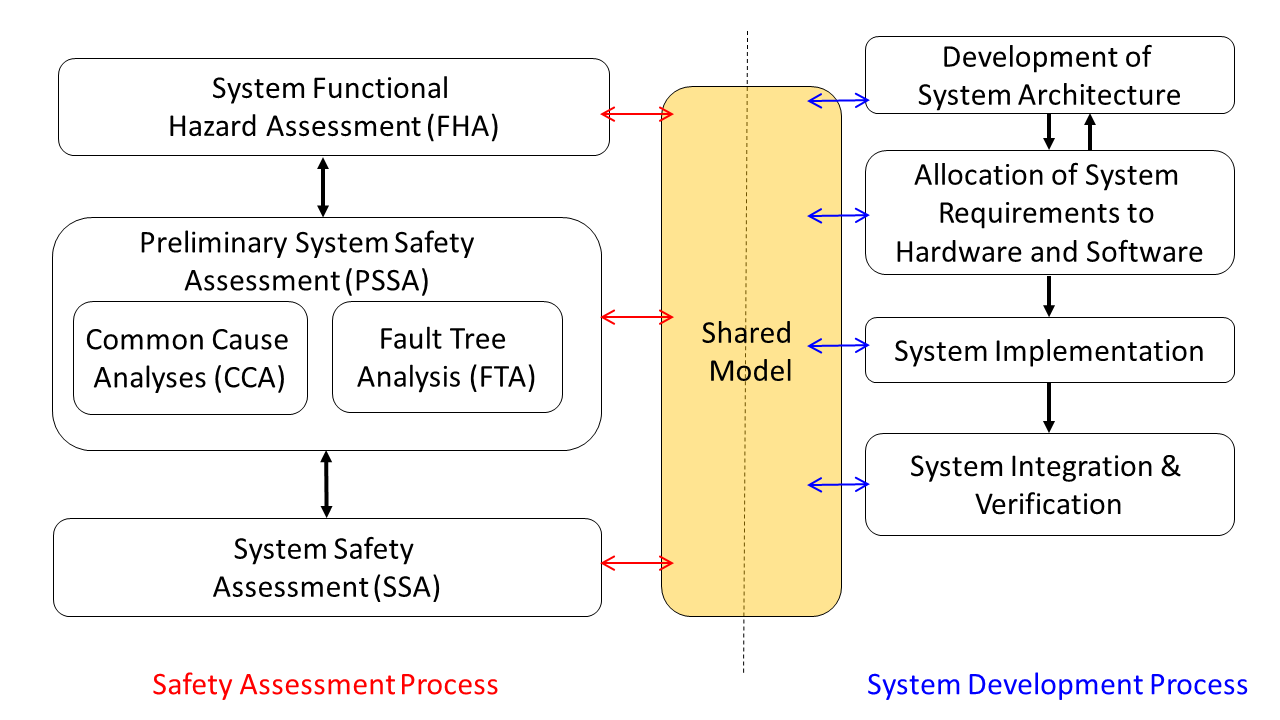
\includegraphics[trim=0 5 0 5,clip,width=0.85\textwidth]{images/process3.png}
	\caption{Use of the Shared System/Safety Model in the ARP4754A Safety Assessment Process}
	\label{fig:proposed_safety_process}
\end{figure}

Industry practitioners have come to realize the benefits of using models in the safety assessment process, and a revision of the ARP4761 to include Model Based Safety Analysis (MBSA) is under way. 

\subsection{Suggested Model Based Safety Assessment Process Supported by Formal Methods}
We propose a model-based safety assessment process backed by formal methods to help safety engineers with early detection of the design issues.  This process uses a single unified model to support both system design and safety analysis; this is shown in Figure~\ref{fig:SACycle1} and is based on the following steps:

\begin{enumerate}
	\item System engineers capture the critical information in a shared model:  high-level hardware and software architecture, nominal behavior at the component level, and safety requirements at the system level.
	\item System engineers use a model checker to check that the safety requirements are satisfied by the nominal design model. 
	\item Safety engineers augment the nominal model with the component failure modes. In addition, safety engineers specify the fault hypothesis for the analysis which corresponds to how many simultaneous faults the system must be able to tolerate.
	\item Safety engineers use a model checker to analyze if the safety requirements and fault tolerance objectives are satisfied by the design in the presence of faults. If the design does not tolerate the specified number of faults (or probability threshold of fault occurrence), then the tool produces counterexamples or minimal sets of fault combinations that can cause the safety requirement to be violated.
	\item The safety engineers examine the results to assess the validity of the fault combinations and the fault tolerance level of the system design. If a design change is warranted, the model will be updated with the latest design change and the above process is repeated.
\end{enumerate}

\begin{figure}[h]
	\begin{center}
		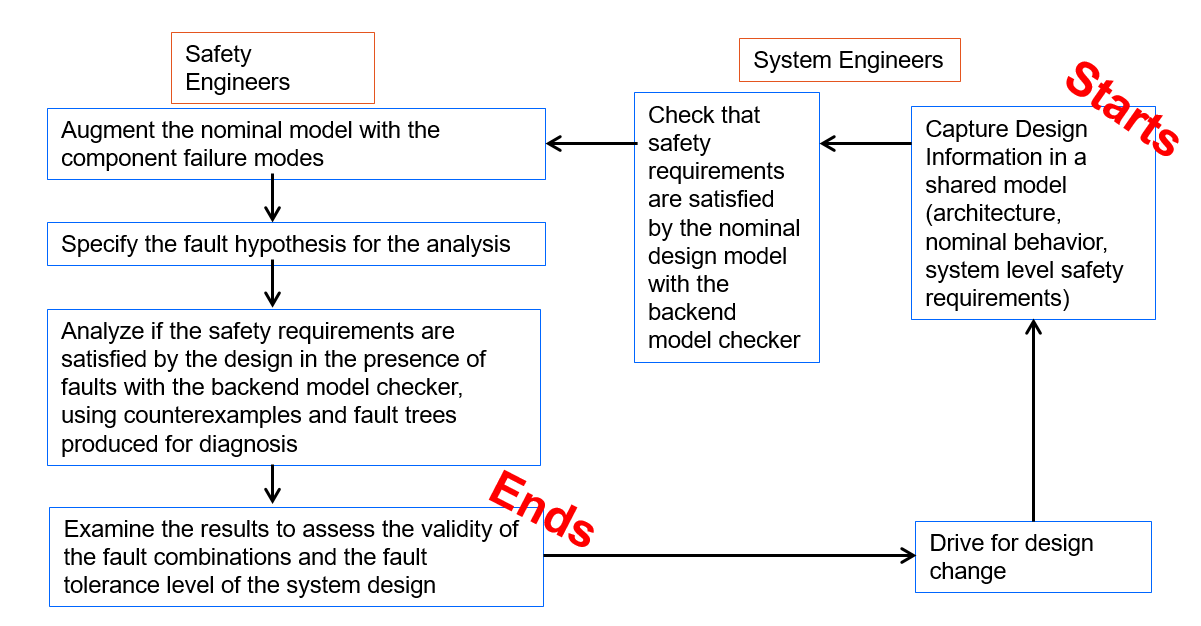
\includegraphics[width=\textwidth]{images/SACycle.PNG}
	\end{center}
	\caption{Proposed Steps of the Safety Assessment Process}
	\label{fig:SACycle1}
\end{figure}

These steps can be viewed as a cyclical process that involves both the system development engineers and the safety engineers of the system. Figure~\ref{fig:SACycle1} shows these steps within the context of the start and end of a project. 

\danielle{Add a bit more information here - pull from the MBSE project for IRAD. Include reasons why this approach is better, how it will help safety analysts, how it benefits the field as a whole. Then lead into the next sections with a statement about model checking, verification, etc.}
subsection{Critical System Development Artifacts}
\label{subsec:crisysArtifacts}












\begin{comment}
ARP4754A, the Guidelines for Development of Civil Aircraft and Systems~\cite{SAE:ARP4754A}, provides guidance on applying development assurance at each hierarchical level throughout the development life cycle of highly-integrated/complex aircraft systems. It has been recognized by the Federal Aviation Administration (FAA) as an acceptable method to establish the assurance process. The safety assessment process is a starting point at each hierarchical level of the development life cycle and is tightly coupled with the system development and verification processes. It is used to show compliance with certification requirements and for meeting a company's internal safety standards. 

ARP4761, the Guidelines and Methods for Conducting Safety Assessment Process on Civil Airborne Systems and Equipment~\cite{SAE:ARP4761},  identifies a systematic means to show compliance. Among the industry accepted safety assessment processes are Preliminary System Safety Assessment (PSSA) and System Safety Assessment (SSA). PSSA evaluates the system design and defines safety requirements. SSA evaluates the implemented system to show that safety requirements defined in the PSSA are in fact satisfied.

A prerequisite of performing the safety assessment is understanding how the system is intended to work, primarily focusing on the integrity of the outputs and the availability of the system. The safety engineers then use the acquired understanding to conduct safety analysis, construct safety analysis artifacts, and compare the results with established safety objectives and requirements.
Typically equipped with the domain knowledge about the system, but not detailed knowledge of how the software applications are designed, practicing safety engineers find it a time consuming and involved process to acquire the knowledge about the behavior of the software applications hosted in a system and its impact on the overall system behavior.
Industry practitioners have come to realize the benefits of using models in the safety assessment process, and a revision of the ARP4761 to include Model Based Safety Analysis (MBSA) is under way.
Figure~\ref{fig:proposed_safety_process} presents our proposed use of a single unified model to support both system design and safety analysis. It describes both system design and safety-relevant information 
that are kept distinguishable and yet are able to interact with each other. The shared model maintains a living model that captures the current state of the system design as it moves through the development lifecycle, allowing all participants of the ARP4754A process to be able to communicate and review the system design. Safety analysis artifacts can be generated directly from the model, 
providing
the capability to more accurately analyze complex systems.

\begin{figure}[t!]
	
	\centering
	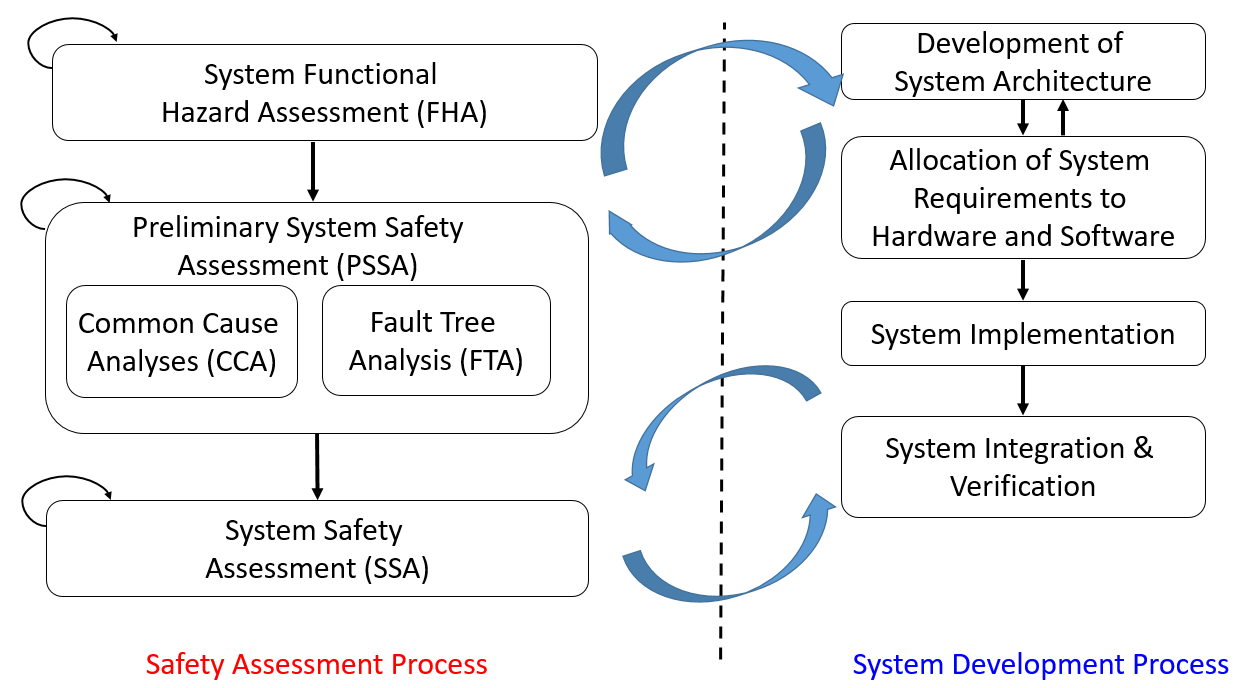
\includegraphics[trim=0 5 0 5,clip,width=0.85\textwidth]{images/process1.png}
	
	\caption{The ARP4754A Safety Assessment Process}
	\label{fig:safety_process}
\end{figure}

\begin{figure}[t!]
	
	\centering
	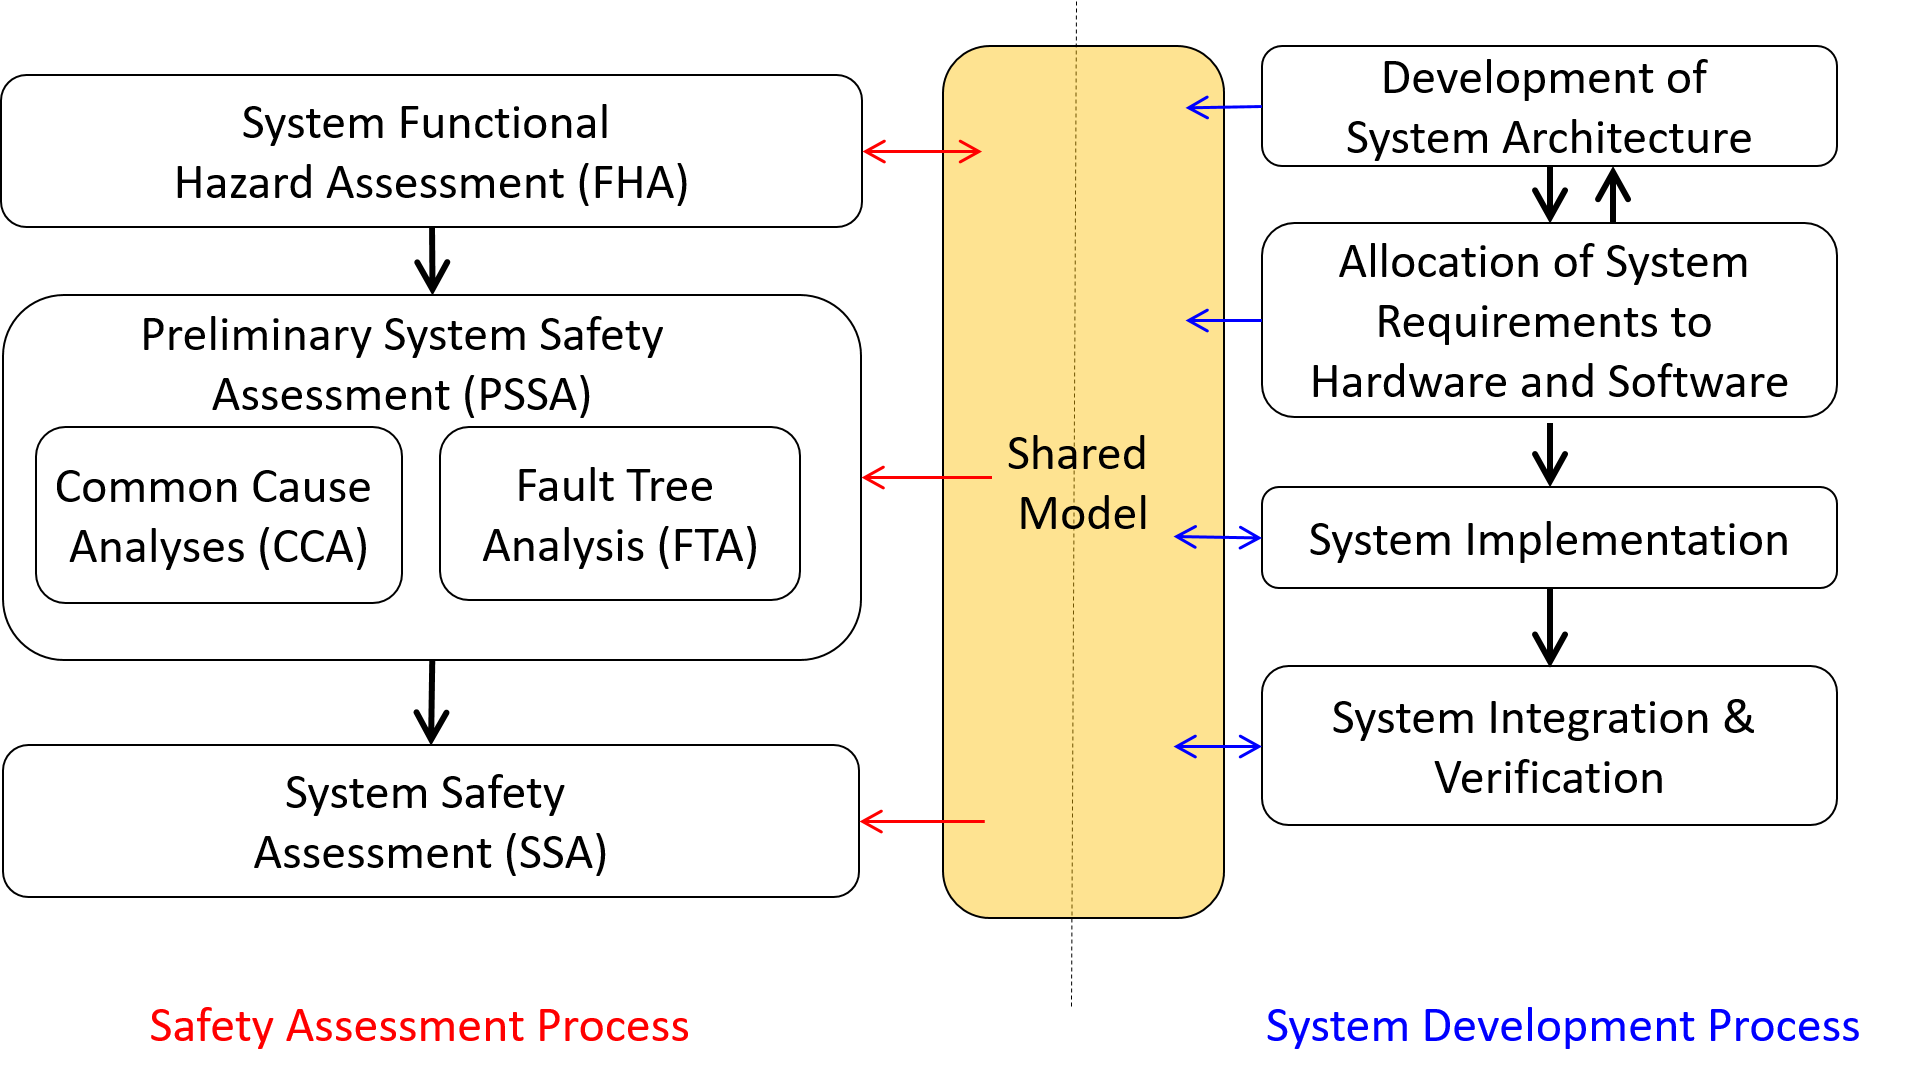
\includegraphics[trim=0 5 0 5,clip,width=0.85\textwidth]{images/process2.png}
	
	\caption{Use of the Shared System/Safety Model in the ARP4754A Safety Assessment Process}
	\label{fig:proposed_safety_process}
\end{figure}
\end{comment}
%\section{Formal Methods in Safety Analysis: A Brief History and the State of the Practice}
\label{sec:modelCheckingInSA}
Safety analysis has traditionally been performed manually, but with the rise of model checking and the improvement of its capabilities, the world of safety analysis began to see its powerful benefits~\cite{hinchey2012industrial, liggesmeyer1998improving, coudert1993fault, Bozzano:2010:DSA:1951720,bozzano2003esacs}. There arose multiple ways of viewing the system and fault models, various ways of automating the capture of safety pertinent information, and a number of tools that addressed various issues that arose. In this section, we discuss the state of the practice and how formal methods has been applied in the domain of safety assessment research.

\subsection{Fault Tree Analysis}
Since the early days of safety engineering, fault tree analysis has been a primary method of determining safety of a system and showing the behavior of the system (with respect to its requirements) in the presence of faults~\cite{0f356f05e72f43018211b36f97c8854a,vesely1981fault}. Fault tree analysis requires one to explore the faults of the system and their effects on system behavior to determine minimal fault configurations (minimal cut sets) that cause violation of requirements. From the beginning of fault tree analysis in the '60's, algorithms worked directly with the fault tree structure to produce MinCutSets~\cite{10020219108,semanderes1971elraft}. As the years progressed, it was clear that this approach could not sufficiently address the problem of computation time. In 1993, Rauzy et al. developed a new approach that converted the fault tree structure into a binary decision diagram (BDD)~\cite{rauzy1993new}. This was a natural way to reduce the Boolean formula into something far more computationally efficient and reduceable to even simpler forms. Numerous algorithms were developed to perform variable ordering and minimization of the BDD; this resulted in better computation of MinCutSets and began the process of automating a complex manual safety analysis task~\cite{sinnamon1997new,bryant1986graph,aralia1996computation,reay2002fault,rauzy2007assessment}. BDDs are still commonly used to perform quantitative and qualitative fault tree analysis~\cite{ge2015quantitative,jiang2018algebraic,banov2019new}.

\subsection{Model Checking in Model Based Safety Analysis}
From the beginnings of model checking, there was a slow increase in its application to the domain of safety analysis, but a few research groups contributed immensely to this branch of study. Separately, these researchers began to contribute to safety analysis through the use of model checking starting in the '90's and are still contributing today (e.g., \cite{reese1997software,signoret1998altarica,chiappini1999formal,cimatti2000industrial}. 

One of the main methods was the abstraction of the system into a formal transition system; this provided a means of defining a precise mathematical model of the system and simplifying mathematical operations through the use of abstraction techniques on the transition system. This helped to shrink the entire state space into something more digestible by computational techniques~\cite{d2008survey}. 

In the early 2000's, model based safety assessment began to make an appearance in literature~\cite{Bozzano:2010:DSA:1951720,Joshi05:Dasc, Joshi05:SafeComp, Joshi07:Hase}. This applied model checking and model based system development to safety analysis at the same time.  In this approach, a safety analysis system model (SASM) is the central artifact in the safety analysis process, and traditional safety analysis artifacts, such as fault trees, are automatically generated by tools that analyze the SASM.

The contents and structure of the SASM differ significantly across different conceptions of MBSA.  We can draw distinctions between approaches along several different axes.  The first is whether they propagate faults explicitly through user-defined propagations, which we call {\em failure logic modeling} (FLM), or {\em explicit propagation}, or through existing behavioral modeling, which we call {\em failure effect modeling} (FEM), or {\em implicit propagation}.  The next is whether models and notations are {\em purpose-built} for safety analysis vs. those that extend {\em existing system models} (ESM).

For FEM approaches, there are several additional dimensions.  One dimension involves whether {\em causal} or {\em non-causal} models are allowed.  Non-causal models allow simultaneous (in time) bi-directional error propagations, which allow more natural expression of some failure types (e.g. reverse flow within segments of a pipe), but are more difficult to analyze.  A final dimension involves whether analysis is {\em compositional} across layers of hierarchically-composed systems or {\em monolithic}.  %Our approach is an extension of AADL (ESM), causal, compositional, mixed FLM/FEM approach.
\danielle{Make a figure here - that will help explain these distinctions.}

This literature overview is not a complete account of all safety analysis model checking tools available either in industry or research, but highlights some of the most influential safety assessment methods and tools currently available. 

\subsubsection{AltaRica}
AltaRica was one of the first model checking tools specifically aimed at safety analysis of critical systems. The first iteration of AltaRica (1.0) performed over a transition system of the model, used dataflow ({\em causal}) semantics, and could capture the hierarchy of a system~\cite{signoret1998altarica}. The key idea was that this transition system (more specifically {\em constraint automata}) could be compiled into Boolean formulae and transformed into a BDD~\cite{point1999altarica}. The literature for performing fault tree analysis over BDDs was rich with algorithms; this was how much of the safety analysis artifacts were generated. The dataflow dialect (AltaRica 1.0) has substantial tool support, including the commercial Cecilia OCAS tool from Dassault~\cite{bieber2004safety}. For this dialect, the safety assessment, fault tree generation, and functional verification can be performed with the aid of NuSMV model checking~\cite{symbAltaRica}.

The most recent language update (AltaRica 3.0) uses non-causal semantics~\cite{prosvirnova2013compilationfaulttrees,PROSVIRNOVA2013127}. Failure states are defined throughout the system and flow variables are updated through the use of assertions~\cite{Bieber04safetyassessment}.  AltaRica 3.0 has support for simulation and Markov model generation through the OpenAltaRica (www.openaltarica.fr) tool suite; it is a {\em FEM}-based, {\em purpose-built}, {\em monolithic} safety analysis language. 

AltaRica 3.0 provides automated fault tree generation by translating the model into a reachability graph and then further compiling it into Boolean formula in order to compute minimal cut sets~\cite{prosvirnova2015automated}. 

\subsubsection{FSAP, xSAP, and COMPASS}
The Formal Safety Analysis Platform (FSAP) was introduced in 2003~\cite{bozzano2003improving} and supported failure mode definitions, safety requirements in temporal logic formulae, automated fault tree construction, and counterexample traces. The platform used NuSMV, a BDD-based model checker~\cite{Cimatti2000}. The system model, written in NuSMV, and the fault model, developed graphically in FSAP, are together translated into a finite state machine and eventually into a BDD; fault tree analysis is performed using BDD algorithms implemented in NuSMV. 

By 2016, the researchers that developed FSAP (Foundation Bruno Kessler, FBK) released a similar tool called xSAP~\cite{DBLP:conf/tacas/BittnerBCCGGMMZ16}. xSAP extends FSAP in many ways: xSAP can handle infinite state machines, it is textual language rather than graphical, allows for richer fault modeling and definitions, and implements more than just BDD computations (e.g., SAT- and SMT-based routines). xSAP was integrated into the COMPASS toolsuite to take advantage of the algorithms it supports. More complex SAT-based algorithms were introduced to bypass the BDD method of minimal cut set generation, namely the ``anytime approximation" algorithms~\cite{CAV2015:BoCiGrMa, mattarei2016scalable}. These algorithms make clever use of bounded model checking algorithms to explore counterexamples provided to the query "the top level event never occurs." These explorations are done such that the cut sets generated are of increasing cardinality which allows for an approximation computation to be given even when the state space is too large to compute all minimal cut sets. These are implemented in xSAP~\cite{CAV2015:BoCiGrMa}.

COMPASS (Correctness, Modeling project and Performance of Aerospace Systems)~\cite{10.1007/978-3-642-04468-7_15} is a mixed {\em FLM/FEM}-based, {\em causal} {\em compositional} tool suite that uses the SLIM language, which is based on a subset of the Architecture Analysis and Design Language (AADL), for its input models~\cite{5185388, criticalembeddedsystems}. In SLIM, a nominal system model and the error model are developed separately and then transformed into an extended system model.  This extended model is automatically translated into input models for the NuSMV model checker~\cite{Cimatti2000, NuSMV}, MRMC (Markov Reward Model Checker)~\cite{Katoen:2005:MRM:1114692.1115230, MRMC}, and RAT (Requirements Analysis Tool)~\cite{RAT}. The safety analysis tool xSAP~\cite{DBLP:conf/tacas/BittnerBCCGGMMZ16} can be invoked in order to generate safety analysis artifacts such as fault trees and FMEA tables~\cite{compass30toolset}.  %COMPASS is an impressive tool suite, but some of the features that make AADL suitable for SW/HW architecture specification: event and event-data ports, threads, and processes, appear to be missing, which means that the SLIM language may not be suitable as a general system design notation (ESM).

\subsubsection{SmartIFlow}
SmartIFlow~\cite{info17:HaLuHo,honig2014new} is a {\em FEM}-based, {\em purpose-built}, {\em monolithic} {\em non-causal} safety analysis tool that describes components and their interactions using finite state machines and events. Verification is done through an explicit state model checker which returns sets of counterexamples for safety requirements in the presence of failures.  SmartIFlow allows {\em non-causal} models containing simultaneous (in time) bi-directional error propagations.  On the other hand, the tools do not yet appear to scale to industrial-sized problems, as mentioned by the authors: ``As current experience is based on models with limited size, there is still a long way to go to make this approach ready for application in an industrial context''~\cite{info17:HaLuHo}.

\subsubsection{SAML}
The Safety Analysis and Modeling Language (SAML)~\cite{Gudemann:2010:FQQ:1909626.1909813} is a {\em FEM}-based, {\em purpose-built}, {\em monolithic} {\em causal} safety analysis language that was developed in 2010.  System models constructed in SAML can be used used for both qualitative and quantitative analyses. It allows for the combination of discrete probability distributions and non-determinism. The SAML model can be automatically imported into several analysis tools like NuSMV~\cite{Cimatti2000}, PRISM (Probabilistic Symbolic Model Checker)~\cite{CAV2011:KwNoPa}, or the MRMC probabilistic model checker~\cite{Katoen:2005:MRM:1114692.1115230}. SAML itself does not provide the formal verification engines, but instead provides a platform to model the safety aspects of a system and then translate this into the input language for a formal verification engine~\cite{Gudemann:2010:FQQ:1909626.1909813}.

\subsubsection{Error Model Annex for AADL}
The SAE (Society of Automotive Engineers) released the
aerospace standard AS5506, named Architecture Analysis and Design Language (AADL), which is a mature industry-standard for embedded systems and has proved to be efficient for architecture modeling~\cite{aerospace2012sae,liu2016research}. AADL supports safety analysis by adding EMA (Error Model Annex) as an extension to the language. EMA allows the user to annotate system hardware and software architectures with hazard, error propagation, failure modes and effects due to failures. Around 2016, Version 2 of the Error Model Annex was released (EMV2)~\cite{EMV2}. EMV2 is an {\em FLM}-based {\em ESM} approach. The faults and error propagations are explicitly defined and the fault tree analysis is performed by traversing propagation paths in reverse to find the original fault that caused the problem~\cite{feiler2017automated}. 



%\section{Formal Methods}
\label{sec:fm}
As the complexity of systems increase, the cost of development and validation consumes more time and resources than ever before; nevertheless, these processes are vital in safety critical systems when the loss of functionality of the system can result in loss of life. Authorities have put in place various thresholds for the likelihood of such events and it is the responsibility of the system developers to show that undesirable events are sufficiently unlikely to occur~\cite{faaSA}. Utilizing the recent advancements in automated formal verification within the validation process has become essential to the certification of critical systems~\cite{deptOfDefense,standard1999,prasad2005survey} and the world of safety analysis began to see its powerful benefits~\cite{hinchey2012industrial, liggesmeyer1998improving, coudert1993fault, Bozzano:2010:DSA:1951720,bozzano2003esacs}. There arose multiple ways of viewing the system and fault models, various ways of automating the capture of safety pertinent information, and a number of tools that addressed practical issues. Formal validation and verification is a proof-based methodology used to assess the correctness of requirements, system design, and implementation. This section provides a background of the formal method techniques that are commonly used in the system development and safety assessment processes.

\subsection{Overview}
Given that this research is focused on model-based system development and safety assessment, we focus our attention onto \emph{model checking} as a method of formal analysis. Model checking is an automatic technique for verifying that system models meet their specified requirements~\cite{clarke2018model}.  Applying model checking to a system design consists of a few main tasks: \emph{modeling}, \emph{formal specification}, and \emph{formal verification}. The digital and mechanical components of a system can be described in abstract form (modeling), and the requirements of the system and of each component can be specified in formal logic (formal specification). Formal verification is demonstrating that the model satisfies its specification using math. The verification of a model takes both the design and the requirement specification into account when analyzing the behavior and interactions of the components. In the sections that follow, we will outline these three major components of model checking and describe the aspects important in this research.

\subsection{Modeling}
\label{sec:modeling}
When modeling a system, the digital and mechanical components are described in abstract form; furthermore, the requirements of the system and of each component can be specified in formal logic. The verification of such models take both the architecture and the requirement specification into account when analyzing the behavior and interactions of the components comprising the system. Throughout the past few decades, numerous modeling languages and tools have been introduced, for example Simulink from MathWorks~\cite{MathWorks}, SCADE from Esterel Technologies~\cite{abdulla2004designing}, and research base languages such as Lustre~\cite{Halbwachs91:IEEE}. Other common modeling languages include SysML~\cite{friedenthal2014practical} and AADL~\cite{FeilerModelBasedEngineering2012}. 

Often, engineers who design safety critical systems model their systems as networks of operators transforming flows of data. At a higher level, this can be represented by block diagrams that group these networks into reusable components. {\em Dataflow} languages allow these models to directly represent the digital control system. Dataflow programming languages have several merits, one of which is that the program is a completely functional model of the system. This feature makes the model well suited to formal verification and program transformation; it also facilitates reuse, because the module will behave the same way in any context into which it is embedded~\cite{joshi2008behavioral}. For this dissertation, we focus our attention on Lustre~\cite{Halbwachs91:IEEE}, a synchronous\footnote{A synchronous language breaks real time into a sequence of instants in which the outputs of the model are computed.} dataflow programming language used in the formal verification portion of this research. Lustre is described in more detail in Section~\ref{sec:lustre}. 




\begin{comment}
\subsubsection{Ordered Binary Decision Diagrams}
A Binary Decision Diagram (BDD) is a data structure used to encode Boolean formulae.
\begin{figure}[htbp]
        \center{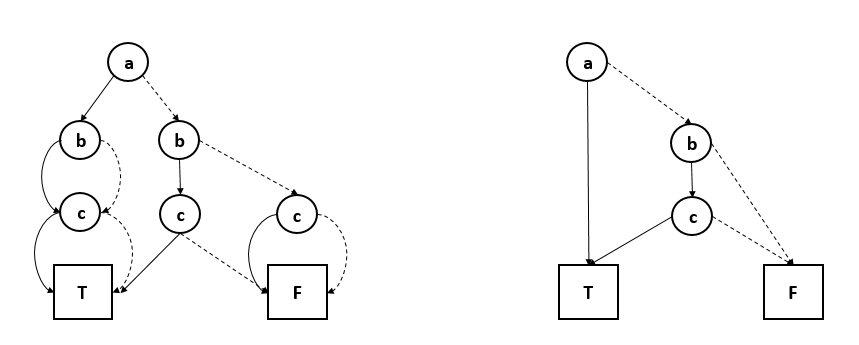
\includegraphics[width=0.8\textwidth] {images/bdd.png}}
        \caption{\label{fig:bdd} Binary Decision Diagrams of the Formula $a \lor (b \land c)$}
\end{figure}
As shown in Figure~\ref{fig:bdd}, it is a rooted, directed, acyclic graph with internal decision nodes and two terminal nodes (\textit{true} and \textit{false}). Each of the decision nodes is labeled with a Boolean variable and has two child nodes, low child and high child. The edge from a node to its low child represents the assignment of \textit{false}, likewise the edge to the high child represents the assignment of \textit{true}. The BDD is called \textit{ordered} if different variables appear in the same order on all paths from the root. Intuitively, following a path from the root to the \textit{true} terminal node represents a valid assignment to the Boolean formula (invalid in the case of ending on the \textit{false} terminal node). 

BDDs are reduced by the removal of isomorphic subgraphs. The BDD shown on the right of Figure~\ref{fig:bdd} is the reduced form of the BDD on the left.
\end{comment}


\subsection{Formal Specification}
\label{sec:formalSpec}
Before we can verify the correctness of a system, we must first specify the properties that the system should have~\cite{clarke2018model}. The formal specification process translates the informal system requirements into a mathematical logic to determine if the system design is correct~\cite{hinchey2012industrial}. This process guarantees an unambiguous description of the requirements, which is not possible when using an informal natural language. The formal definition of system requirements includes the system design and its expected behavior as well as the assumptions on the environment in which the system is expected to operate. A design or implementation can never be considered correct in isolation; it is only correct with respect to the specifications. The expected behavior, system design, and environmental assumptions change and are refined as the system goes through the various stages of development~\cite{lamsweerde2000formal}. A commonly used method of specification is \emph{temporal logic}. Temporal logics are useful for specifying complex system requirementss, because they can describe the ordering of events in time without introducing time explicitly. 

\subsubsection{Linear Temporal Logic}
Temporal logic can be used to express properties of reactive systems~\cite{Bozzano:2010:DSA:1951720}. System properties are usually classified into two main categories: {\em safety properties} and {\em liveness properties}. Safety properties express the idea that ``nothing bad ever happens" where liveness properties state that ``something good will eventually happen." 

An example of a safety property is: ``it is never the case that the brake pedal is pressed and no hydraulic pressure is supplied at the wheel." A liveness property, on the other hand, could state: ``eventually the process will complete its execution." 

Traditionally, two types of temporal logic are used in model checking; Computational Tree Logic (CTL), which is based on a branching time logic model, and Linear Temporal Logic (LTL), based on a linear representation of time. This research will focus on LTL. 

An LTL formula is built from a set of atomic propositions, logical operators, and basic temporal operators. The formula is evaluated over a linear path or sequence of states, $s_0, s_1, ..., s_i ,s_{i+1},...$. The following temporal operators are provided:
\begin{itemize}
    \item Globally (\textbf{G}): $G_p$ is true in a state $s_i$ if and only if $p$ is true in all states $s_j$ with $j \geq i$.
    
    \item Finally (\textbf{F}): $F_p$ is true in state $s_i$ if and only if $p$ is true in some state $s_j$ with $j \geq i$.
    
    \item Next (\textbf{X}): $X_p$ is true in state $s_i$ if and only if $p$ is true in the state $s_{i+1}$. 
    
    \item Until (\textbf{U}): $pUq$ is true in state $s_i$ if and only if $q$ is true in some state $s_j$ with $j \geq i$ and $p$ is true in all states $s_k$ such that $i \leq k < j$.
\end{itemize}

Other temporal operators can be defined on the basis of the operators above~\cite{sistla1985complexity}. Formal definitions and more information on LTL and CTL can be found in a number of research works~\cite{Bozzano:2010:DSA:1951720, clarke2018model}.

\subsection{Formal Verification} 
\label{sec:formalVer}
Once we have specified the important properties (formal specification), then a formal model for the system is created; this model captures the properties that must be considered to establish correctness~\cite{clarke2018model}; this process is referred in this dissertation as \emph{formal verification}. Formal verification is the use of proof methods to show that given the environmental assumptions stated in the formal specification, the formal design of the system meets the requirements. The problem can be reduced to that of property checking: given a program $P$ and a specific property, does the program satisfy the given property~\cite{fitting2012first}.  

Model checking was introduced in the early 1980s and consists of exploring the states and transitions of a model~\cite{clarke1981design,queille1982specification}. By representing the system abstractly, a possibly infinite state space is reduced to a finite model.~\cite{d2008survey}. The proofs are generated over an abstract mathematical model of the system, such as finite state machines, labeled transition systems, or timed automata. It takes as input a model of a system and the properties written in formal logic, then explores the state space of the system to determine if the model violates the properties~\cite{clarke2018model,fraser2009testing}. In recent years, model checking takes advantage of abstraction techniques specific to a domain to consider multiple states or transitions in a single operation; this lessens computation time considerably~\cite{d2008survey}. Nevertheless, the biggest limiting factor of model checking is scalability and much of the recent research in this area attempts to address this problem~\cite{clarke2018model}.

Deductive methods of verification consists of generating proof obligations from the specifications of the system and using these obligations in a theorem prover setting. Automated theorem provers have the main objective to show that some statement (conjecture) is a logical consequence of other statements (the axioms and hypotheses). The rules of inference are given as are the set of axioms and hypotheses~\cite{d2008survey,fitting2012first}. Deductive methods of verification include automated theorem provers (e.g., Coq~\cite{coq}, Isabelle~\cite{isabelle}) and satisfiability modulo theories (e.g., SMTInterpol~\cite{smtInterpol}, Z3~\cite{z3}, Yices~\cite{yices}). 



